\documentclass[aspectratio=149]{beamer}


\usepackage[utf8]{inputenc}
\usepackage[T2A]{fontenc}
\usepackage[russian,english]{babel}


\usepackage{outlines}

\usepackage{colortbl}

\definecolor{ltgrey}{rgb}{0.85,0.85,0.85}
\definecolor{ltblue}{RGB}{101,147,245}
\definecolor{dkblue}{rgb} {0,   0.1, 0.6}
\definecolor{dkred} {rgb} {0.6, 0.1, 0}
\renewcommand{\r}[1]{\ensuremath{\textcolor{dkred}{#1}}}
\renewcommand{\b}[1]{\ensuremath{\textcolor{dkblue}{#1}}}

\usepackage{xparse}
\usepackage{tikz}
\usetikzlibrary{tikzmark}
\usetikzlibrary{positioning}
\usetikzlibrary{calc}
\usetikzlibrary{arrows}
\usetikzlibrary{decorations.pathmorphing,decorations.markings}
\usetikzlibrary{shapes}
\usetikzlibrary{patterns}
\usetikzlibrary{automata}

\tikzset{
c/.style={
  circle,solid,
  inner sep=0pt,
  %text width=1mm,
  minimum width=7mm,
  align=center,
  draw=black,
  fill=white
  }
}

\newcommand*{\yellowemph}[1]{%
  \tikz[baseline=(X.base)] \node[rectangle, fill=yellow, inner sep=0mm] (X) {#1};%
}

\newcommand*{\rus}[1]{%
  %\textcolor{black}{
  \textit{#1}
  %}
}

\newcommand{\tool}[1]{\texttt{#1}}
\newcommand*{\fx}{\ensuremath{\mathbf{x}}}%x}}}
\newcommand*{\fv}{\ensuremath{\mathbf{v}}} %v}}}
\newcommand{\defeq}{\ensuremath{=}}%\coloneqq}}%\Leftrightarrow}}%\triangleq}}

\usepackage{multicol}

\usepackage{fancyvrb}%fancy verbatim
%\makeatletter
%\newcommand{\verbatimfont}[1]{\renewcommand{\verbatim@font}{\ttfamily\scriptsize#1}}
%\makeatother
% redefine \VerbatimInput
\RecustomVerbatimCommand{\VerbatimInput}{VerbatimInput}{fontsize=\scriptsize}

\usepackage{pmboxdraw}
\usepackage{newunicodechar}
\newunicodechar{└}{\textSFii}
\newunicodechar{├}{\textSFviii}
\newunicodechar{─}{\textSFx}


\usepackage[export]{adjustbox} % loads also graphicx

%\usepackage{../inc/listingset}
\usepackage{listings}
\lstset{escapeinside={[*}{*]}}

\usepackage{subcaption}
\usepackage[font=scriptsize]{caption}
\setlength{\abovecaptionskip}{5pt plus 0pt minus 2pt} % Chosen fairly arbitrarily

\usepackage[backend=biber]{biblatex}
\addbibresource{../bib/ms-thesis.bib}

\usepackage{array}
%\usepackage{xcolor}

\usepackage{hyphenat} % for using \nohyphens
%\usepackage{multirow} %Used for tables with merged cells
%\usepackage{collcell} %pdflatex.exe hangs without this one

\usepackage{booktabs}% http://ctan.org/pkg/booktabs
\newcommand{\tabitem}{~~\llap{\textbullet}~~}

\addtolength{\tabcolsep}{-3pt}
\setlength{\leftmargini}{10pt}
%\RequirePackage{aaltologo}
%\RequirePackage{beamercolorthemeAalto}
%\RequirePackage{beamerthemeAalto}

% There are many different themes available for Beamer. A comprehensive
% list with examples is given here:
% http://deic.uab.es/~iblanes/beamer_gallery/index_by_theme.html
% You can uncomment the themes below if you would like to use a different
% one:
%\usetheme[school={SCI}]{Aalto}
%\usetheme{AnnArbor}
%\usetheme{Antibes}
%\usetheme{Bergen}
%\usetheme{Berkeley}
%\usetheme{Berlin}
%\usetheme{Boadilla}
\usetheme{boxes}
%\usetheme{CambridgeUS}
%\usetheme{Copenhagen}
%\usetheme{Darmstadt}
%\usetheme{default}
%\usetheme{Frankfurt}
%\usetheme{Goettingen}
%\usetheme{Hannover}
%\usetheme{Ilmenau}
%\usetheme{JuanLesPins}
%\usetheme{Luebeck}
%\usetheme{Madrid}\colorbox{yellow}
%\usetheme{Malmoe}
%\usetheme{Marburg}
%\usetheme{Montpellier} %!
%\usetheme{PaloAlto}
%\usetheme{Pittsburgh}
%\usetheme{Rochester}
%\usetheme{Singapore}
%\usetheme{Szeged}
%\usetheme{Warsaw}

%\beamertemplatenavigationsymbolsempty  %no navigation bar
%\setbeamertemplate{footline}[frame number]
%\setbeamertemplate{headline}{}

\addtobeamertemplate{navigation symbols}{}{%
    \usebeamerfont{footline}%
    \usebeamercolor[fg]{footline}%
    \hspace{1em}%
    \insertframenumber%/\inserttotalframenumber
}

%\setbeamercovered{transparent}
%\setbeamertemplate{footline}{}


%\setbeamertemplate{page number in head/foot}[framenumber]

%\setbeamertemplate{frametitle}[default][left]
      
%\titlegraphic{\includegraphics[height=1cm,width=2cm]{logo1}}
%\titlegraphicii{\includegraphics[height=1cm,width=2cm]{logo2}}
\title{\nohyphens{\textbf{Automated~Analysis~of~Weak~Memory~Models}}}

% A subtitle is optional and this may be deleted
%\subtitle{Optional Subtitle}
\author{\textbf{Artem Yushkovskiy}\inst{1,2} \\ 
{\scriptsize MSc Candidate}
\\ \vspace{1em}
{\footnotesize\raggedleft Supervisors: \textbf{Assoc. Prof. Keijo Heljanko}\inst{1} \newline
\hphantom{Supervis} \textbf{Docent Igor I. Komarov}\inst{2} }
}%\small
%{\footnotesize%\raggedleft%does not work
%Supervisor 1: Assoc. Prof. Keijo Heljanko\inst{1} \newline
%Supervisor 2: Docent Igor I. Komarov\inst{2}
%}


\institute
{
  \inst{1}%
  \textbf{Aalto University} (Espoo, Finland) \\
  Department of Computer Science, \\
  School of Science
  \and
  \inst{2}%
  \textbf{ITMO University} (Saint Petersburg, Russia) \\
  Faculty of Information Security \\
  and Computer Technologies
}

\date{\scriptsize Espoo, Saint Petersburg, 2018}
% - Either use conference name or its abbreviation.
% - Not really informative to the audience, more for people (including
%   yourself) who are reading the slides online

%\subject{Computer Science}
% This is only inserted into the PDF information catalog. Can be left
% out. 

% If you have a file called "university-logo-filename.xxx", where xxx
% is a graphic format that can be processed by latex or pdflatex,
% resp., then you can add a logo as follows:

%\pgfdeclareimage[height=0.5cm]{university-logo}{}
%\logo{\pgfuseimage{university-logo}}

% Delete this, if you do not want the table of contents to pop up at
% the beginning of each subsection:
%\AtBeginSection[]
%{
%  \begin{frame}<beamer>{Outline}
%    \tableofcontents[currentsection]%,currentsubsection]
%  \end{frame}
%}



% Let's get started
\begin{document}
%\beamertemplatenavigationsymbolsempty %remove navigation bar

\begin{frame}
  \titlepage
\end{frame}

%\begin{frame}{Outline}
%  \tableofcontents
%\end{frame}




%\section{Introduction}
%\subsection{The problem}


\begin{frame}{Task statement \rus{(Цель работы)}}
\begin{itemize}
\item Improve the proof-of-concept memory model-aware analysis tool \texttt{Porthos}~\cite{Porthos17a} by extending support for the input language.
\end{itemize}
\end{frame}


\begin{frame}{Task specification \rus{(Задачи работы)}}
\begin{itemize}
\item Study the general framework for memory model-aware analysis of concurrent programs~\cite{alglave2010shared};
\item Review existing tools for memory model-aware analysis;
%\item Examine the architecture of \texttt{Porthos}, its strengths and weaknesses;
%\item Design a new architecture for \texttt{PorthosC} that allow to extend the input language to the (large subset of) C language, be robust, transparent, efficient and extensible.
\item Develop a \textit{C compiler infrastructure} as a part of an abstract interpretation engine for the new tool \tool{PorthosC};
\item Improve the SMT-encoding scheme for an \textit{arbitrary control-flow};
\item Enhance performance, extensibility, reliability and maintainability of the tool.
\end{itemize}
\end{frame}


%\subsection{The background: weak memory model-aware analysis}

\begin{frame}{Verification of concurrent software} {Motivating example: Write-write reordering (compiler  relaxations)}
%1) mckenney  http://www.rdrop.com/users/paulmck/scalability/paper/whymb.2010.06.07c.pdf
%2) http://preshing.com/20120515/memory-reordering-caught-in-the-act/
\begin{table}
\centering
\ttfamily
\begin{tabular}{ |>{\color{dkblue}}l | >{\color{dkred}}l| }
\hline
\multicolumn{2}{|c|}{ \{ x=0; y=0; \}} \tabularnewline \hline
P & Q \\ \hline
\tikzmark{p0}$p_0$: $x \leftarrow 1$   & $q_0$: $y \leftarrow 1$\tikzmark{q0} \\
\tikzmark{p1}$p_1$: $r_p \leftarrow y$ & $q_1$: $r_q \leftarrow x$\tikzmark{q1} \\
\hline
\multicolumn{2}{|c|}{ exists ($\b{r_p}=0 \land \r{r_q}=0$) } \\
\hline
\end{tabular}
\end{table}

\onslide<2->
\begin{minipage}{.25\textwidth}
\small
\begin{table}
\only<1>{\caption*{~\\~}}
\only<2>{\caption*{Single thread\\(no concurrency)}}
\only<3>{\caption*{Sequential Consistency\\(classical concurrency)}}
\only<4->{\caption*{~\\~}}
\only<4->{
  \begin{tikzpicture}[overlay, remember picture]
    \draw [<->,thick,red,looseness=3] ([xshift=-5pt,yshift=3pt]{pic cs:p0}) to[bend right=90] ([xshift=-5pt]{pic cs:p1});
    \draw [<->,thick,red,looseness=3] ([xshift=8pt,yshift=3pt]{pic cs:q0}) to[bend left=90] ([xshift=5pt]{pic cs:q1});
  \end{tikzpicture}%
}
%"A multiprocessor is sequentially consistent if the result of any
%execution is the same as some sequential order, and within any
%processor, the operations are executed in program order"
%– Lamport, 1979
\begin{tabular}{ l r }
$\b{p_0}, \b{p_1}, \r{q_0}, \r{q_1}$ & $(\b{0}; \r{1})$ \\
$\r{q_0}, \r{q_1}, \b{p_0}, \b{p_1}$ & $(\b{1}; \r{0})$
\onslide<3->
\\
$\b{p_0}, \r{q_0}, \b{p_1}, \r{q_1}$ & $(\b{1}; \r{1})$ \\
$\b{p_0}, \r{q_0}, \r{q_1}, \b{p_1}$ & $(\b{1}; \r{1})$ \\
$\r{q_0}, \b{p_0}, \b{p_1}, \r{q_1}$ & $(\b{1}; \r{1})$ \\
$\r{q_0}, \b{p_0}, \r{q_1}, \b{p_1}$ & $(\b{1}; \r{1})$ \\
\end{tabular}
\end{table}
\end{minipage}
%
\onslide<4->
\begin{minipage}{.6\textwidth}
\small
%"delay the effect of a store past any load from a different location."
\begin{table}
%http://events17.linuxfoundation.org/sites/events/files/slides/dbueso-elc2016-membarriers-final.pdf
%SPARC, x86 (Intel, AMD)
%Similar to SC, but:
%‒ Loads may be reordered with writes.
%Relaxed Models
% Arbitrary reorder limited only by explicit memorybarrier
%instructions.
\caption*{Total Store Order\\(e.g., x86)}
\begin{tabular}{ | l r | l r | l r } % >{\columncolor{ltgrey}}
$\underline{\b{p_1}}, \underline{\b{p_0}}, \r{q_0}, \r{q_1}$ & $(\b{0}; \r{1})$  &  $\b{p_0}, \b{p_1}, \underline{\r{q_1}}, \underline{\r{q_0}}$ & $(\b{0}; \r{1})$  &  $\underline{\b{p_1}}, \underline{\b{p_0}}, \underline{\r{q_1}}, \underline{\r{q_0}}$ & $(\b{0}; \r{1})$ \\
$\r{q_0}, \r{q_1}, \underline{\b{p_1}}, \underline{\b{p_0}}$ & $(\b{1}; \r{0})$  &  $\underline{\r{q_1}}, \underline{\r{q_0}}, \b{p_0}, \b{p_1}$ & $(\b{1}; \r{0})$  &  $\underline{\r{q_1}}, \underline{\r{q_0}}, \underline{\b{p_1}}, \underline{\b{p_0}}$ & $(\b{1}; \r{0})$ \\
$\underline{\b{p_1}}, \r{q_0}, \underline{\b{p_0}}, \r{q_1}$ & $(\b{0}; \r{1})$  &  $\b{p_0}, \underline{\r{q_1}}, \b{p_1}, \underline{\r{q_0}}$ & $(\b{0}; \r{1})$  &  $\underline{\b{p_1}}, \underline{\r{q_1}}, \underline{\b{p_0}}, \underline{\r{q_0}}$ & {\only<5->\yellowemph{$(\b{0}; \r{0})$}} \\
$\underline{\b{p_1}}, \r{q_0}, \r{q_1}, \underline{\b{p_0}}$ & $(\b{0}; \r{1})$  &  $\b{p_0}, \underline{\r{q_1}}, \underline{\r{q_0}}, \b{p_1}$ & $(\b{1}; \r{1})$  &  $\underline{\b{p_1}}, \underline{\r{q_1}}, \underline{\r{q_0}}, \underline{\b{p_0}}$ & {\only<5->\yellowemph{$(\b{0}; \r{0})$}} \\
$\r{q_0}, \underline{\b{p_1}}, \underline{\b{p_0}}, \r{q_1}$ & $(\b{1}; \r{1})$  &  $\underline{\r{q_1}}, \b{p_0}, \b{p_1}, \underline{\r{q_0}}$ & {\only<5->\yellowemph{$(\b{0}; \r{0})$}}  &  $\underline{\r{q_1}}, \underline{\b{p_1}}, \underline{\b{p_0}}, \underline{\r{q_0}}$ & {\only<5->\yellowemph{$(\b{0}; \r{0})$}} \\
$\r{q_0}, \underline{\b{p_1}}, \r{q_1}, \underline{\b{p_0}}$ & $(\b{1}; \r{0})$  &  $\underline{\r{q_1}}, \b{p_0}, \underline{\r{q_0}}, \b{p_1}$ & $(\b{1}; \r{0})$  &  $\underline{\r{q_1}}, \underline{\b{p_1}}, \underline{\r{q_0}}, \underline{\b{p_0}}$ & {\only<5>\yellowemph{$(\b{0}; \r{0})$}} \\
\end{tabular}
\end{table}
\end{minipage}

\end{frame}



\begin{frame}{Verification of concurrent software} {Motivating example: Store buffering (hardware relaxations)}
\begin{center}
\scalebox{0.75}{
\ttfamily
\begin{tabular}{ |>{\color{dkblue}}l | >{\color{dkred}}l| }
\hline
\multicolumn{2}{|c|}{ \{ x=0; y=0; \}} \tabularnewline \hline
P & Q \\ \hline
$p_0$: $x \leftarrow 1$   & $q_0$: $y \leftarrow 1$\\
$p_1$: $r_p \leftarrow y$ & $q_1$: $r_q \leftarrow x$\\
\hline
\multicolumn{2}{|c|}{ exists ($\b{r_p}=0 \land \r{r_q}=0$) } \\
\hline
\end{tabular}
}
\end{center}

\begin{figure}
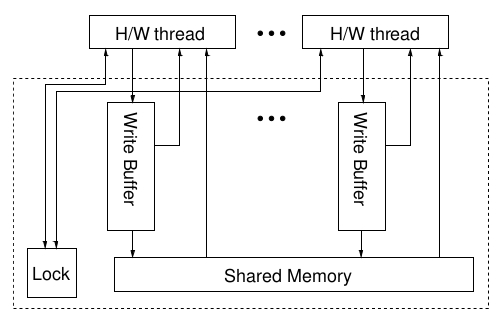
\includegraphics[scale=0.37]{img/x86-arch-full.png}
\caption{An x86-TSO abstract machine~\cite{sewell2010x86}}
\only<2->{
    \begin{tikzpicture}[overlay]
    \node at (0.1, 3.1) {\fcolorbox{yellow}{yellow}{
        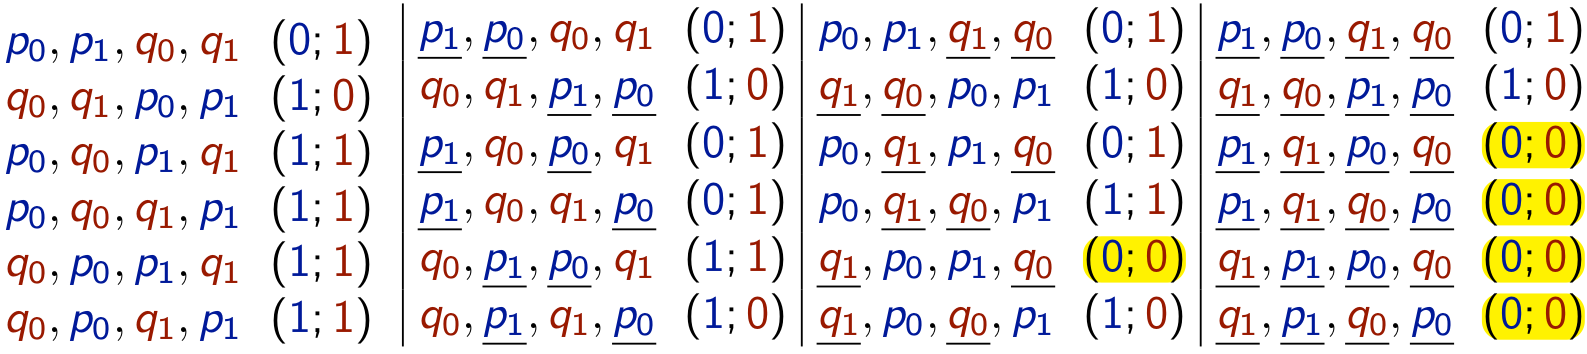
\includegraphics[scale=0.2]{img/table.png}} };
    \end{tikzpicture}
}
\end{figure}

\end{frame}





\begin{frame}{Weak memory model-aware analysis} {Event-based program representation}

\begin{itemize}
  \addtolength{\tabcolsep}{0pt}
  \item \textbf{Event} $\in \mathbb{E}$, a low-level primitive operation:
    \begin{itemize}
      \item \textit{memory event} $\in \mathbb{M} = \mathbb{R} \cup \mathbb{W}$: access to a local/shared memory, \\
      \item \textit{computational event} $\in \mathbb{C}$: computation over local memory, and \\
      \item \textit{barrier event} $\in \mathbb{B}$: synchronisation fences;
     \end{itemize}
  \item \textbf{Relation} $\subseteq \mathbb{E} \times \mathbb{E}$: 
    \begin{itemize}
    \item \textit{basic relations}:%, computed from the program model:
      \begin{itemize}
        \item \textit{program-order} relation $\texttt{po} \subseteq \mathbb{E} \times \mathbb{E}$: (control-flow),
        \item \textit{read-from} relation $\texttt{rf} \subseteq \mathbb{W} \times \mathbb{R}$: (data-flow), and
        \item \textit{coherence-order} relation $\texttt{co} \subseteq \mathbb{W} \times \mathbb{W}$: (data-flow);
      \end{itemize}
    \item \textit{derived relations}:%, computed from the basic relations using the following operators:
      \begin{itemize}
        \item \textit{union} \texttt{r1\,|\,r2},
        \item \textit{sequence} \texttt{r1} ; \texttt{r2},
        %\item \textit{inverse} \texttt{r}\^{\texttt{-1}},
        \item \textit{transitive closure} \texttt{r+},
        \item $\cdots$;
      \end{itemize}
    \end{itemize}
  %\item \textbf{Candidate execution}, a sequence of guesses of relations;
  \item \textbf{Assertion} over relations or sets of events: 
    \begin{itemize}
    \item \textit{acyclicity}, \textit{irreflexivity} or \textit{emptiness} 
    \end{itemize}
\end{itemize}

\end{frame}



\begin{frame}{Weak memory model-aware analysis} {Testing candidate executions}
\vspace{10pt}
\begin{minipage}{.33\linewidth}
\hfill
\end{minipage}
%
\noindent\begin{minipage}{.39\linewidth}
\scalebox{0.65}{
\ttfamily
\begin{tabular}{ |>{\color{dkblue}}l | >{\color{dkred}}l| }
\hline
\multicolumn{2}{|c|}{ \{ x=0; y=0; \}} \tabularnewline \hline
P & Q \\ \hline
$p_0$: $x \leftarrow 1$   & $q_0$: $y \leftarrow 1$\\
$p_1$: $r_p \leftarrow y$ & $q_1$: $r_q \leftarrow x$\\
\hline
\multicolumn{2}{|c|}{ exists ($\b{r_p}=0 \land \r{r_q}=0$) } \\
\hline
\end{tabular}
}
\end{minipage}
%
\noindent\begin{minipage}{.23\linewidth}
\only<2->{
\scriptsize
SC model: \\
... \\
\texttt{fr = (rf\^\,-1; co)} \\
\color{red}\texttt{acyclic(fr $\cup$ po)}
}
\end{minipage}
\vspace{-5pt}
\only<1>{
\begin{figure}
%\centering
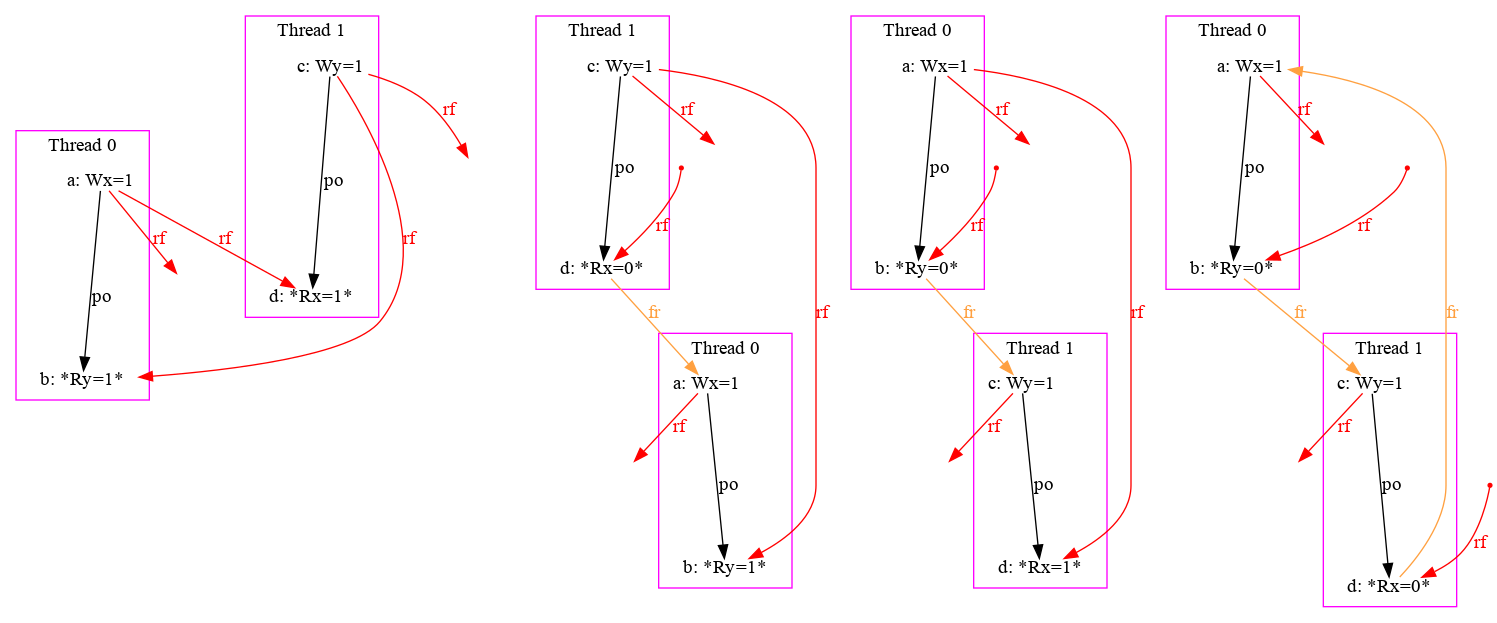
\includegraphics[width=\linewidth]{img/candidate.png}
\caption{The four candidate executions allowed under x86-TSO}
\end{figure}
}
\only<2->{
\begin{figure}
%\centering
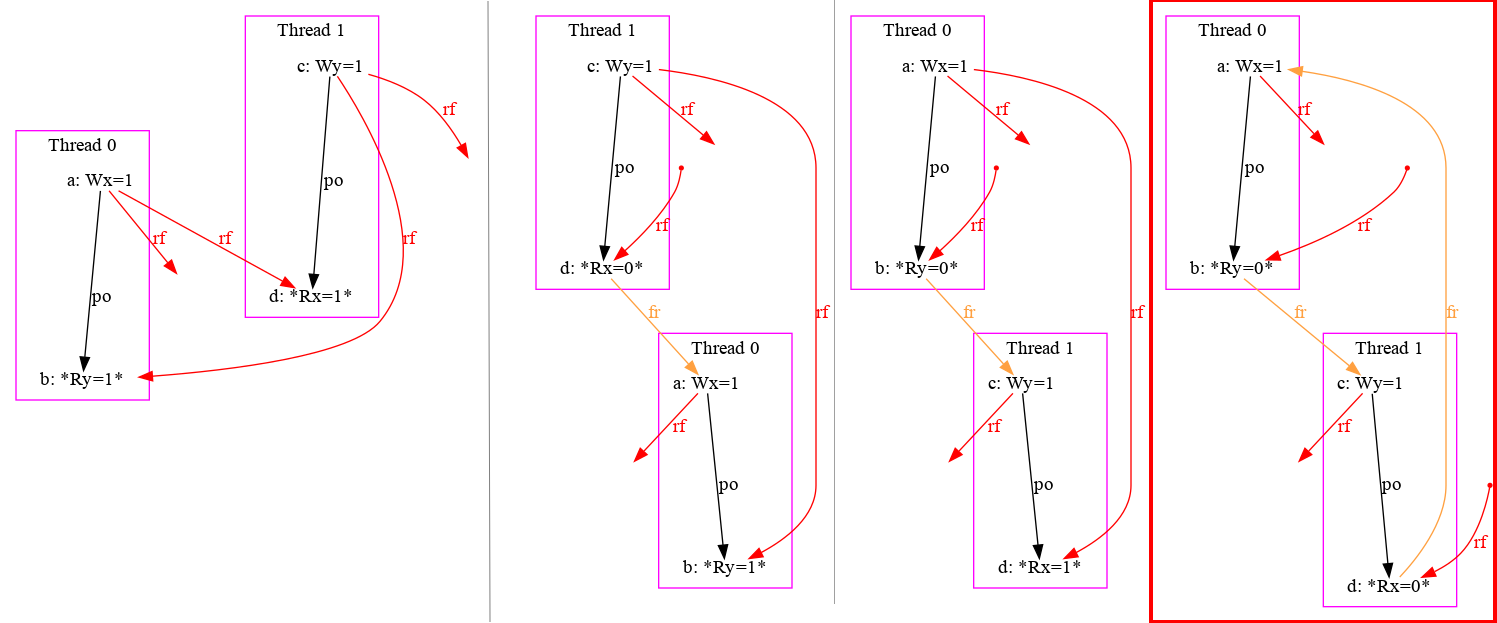
\includegraphics[width=\linewidth]{img/candidate-red.png}
\caption{The four candidate executions allowed under x86-TSO}
\end{figure}
}
\only<3>{
  \begin{tikzpicture}[overlay]
  \node at (6.1, 4.1) {\fcolorbox{yellow}{yellow}{
    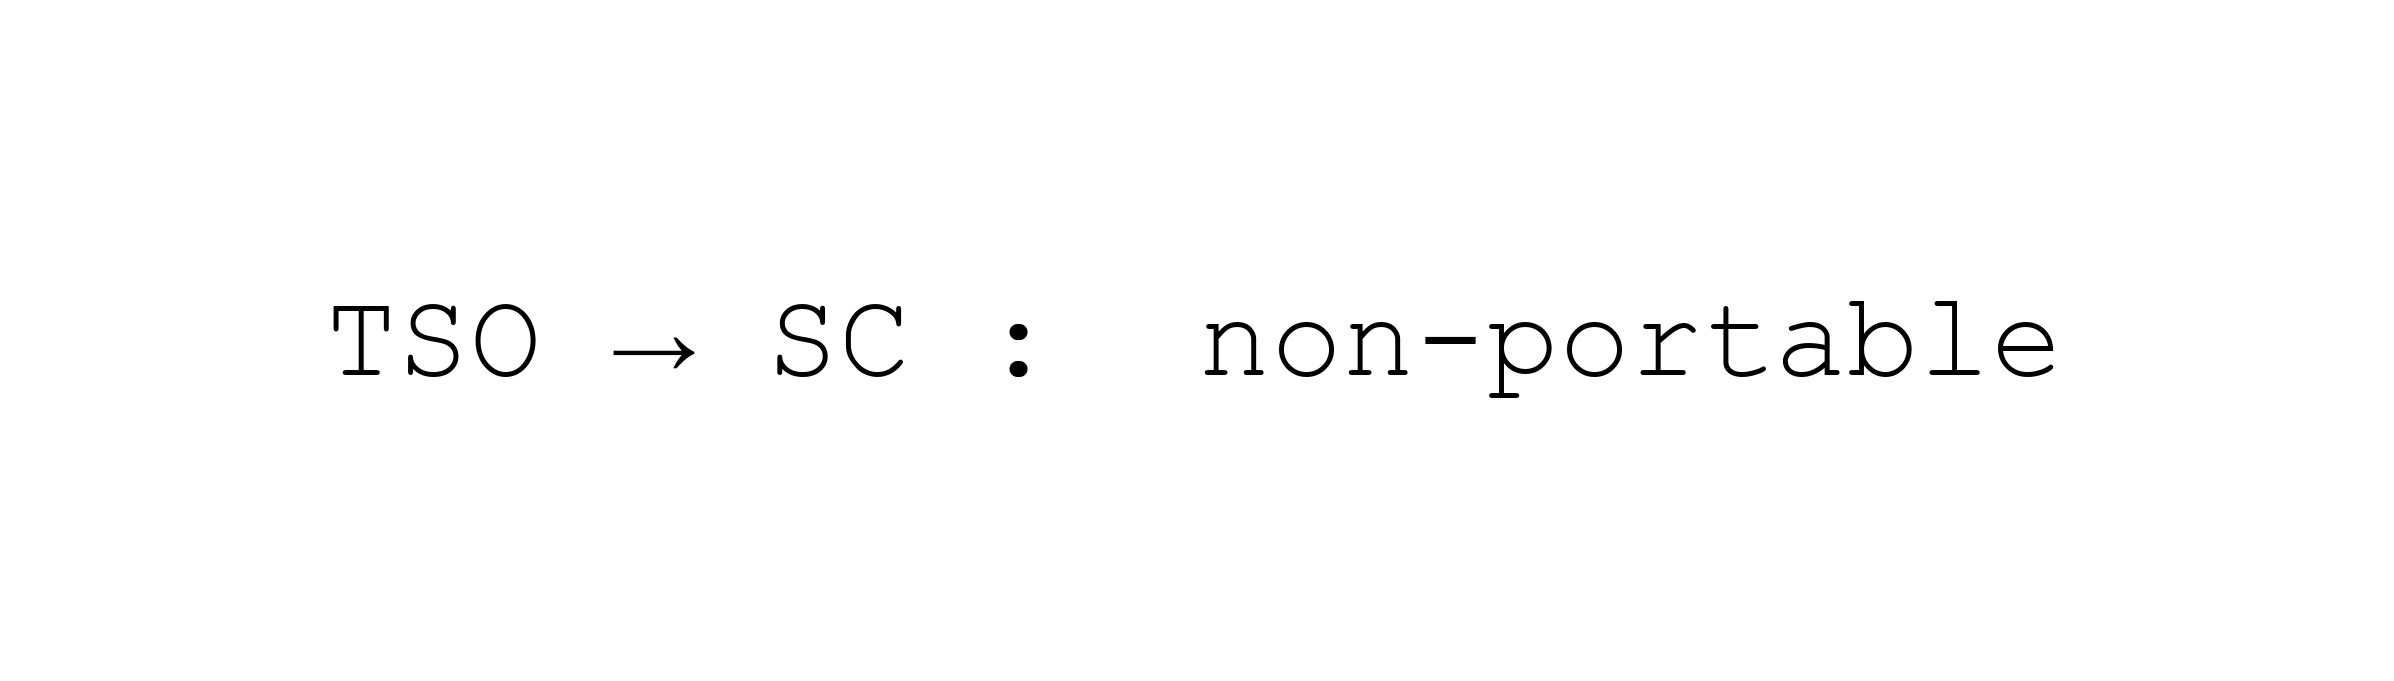
\includegraphics[scale=0.11]{img/non-portable.png}} };
  \end{tikzpicture}
}

\end{frame}




\begin{frame}<presentation:0>{Tools for memory model-aware analysis}
\begin{itemize}
\item \texttt{diy} tool suite:
  \begin{itemize}
  \item \tool{diy}, \tool{diycross} and \tool{diyone}, litmus tests generators,
  \item \tool{litmus}, a litmus test concrete executor, and 
  \item \tool{herd}, a weak memory model simulator;
  \end{itemize}
%\item the stateless model checkers (\tool{CHESS}~\cite{musuvathi2008fair}, \tool{Nidhugg}~\cite{abdulla2017stateless}); %TODO: description of statelessses
\item the stateless model checkers (\tool{CHESS}, \tool{Nidhugg}); %TODO: description of statelessses
\item the tool for automated synthesis of the synchronisation primitives \tool{musketeer};
\item the instrumenting compiler \tool{goto-cc} which is a part of \tool{CBMC} model checker;
\item the tool \texttt{Porthos} for analysing the portability of the C programs;
\item and others.
\end{itemize}
\end{frame}



\begin{frame}{Portability analysis} {The \tool{Porthos} tool}
\begin{minipage}{.49\textwidth}
\only<1->{
  \begin{figure}
  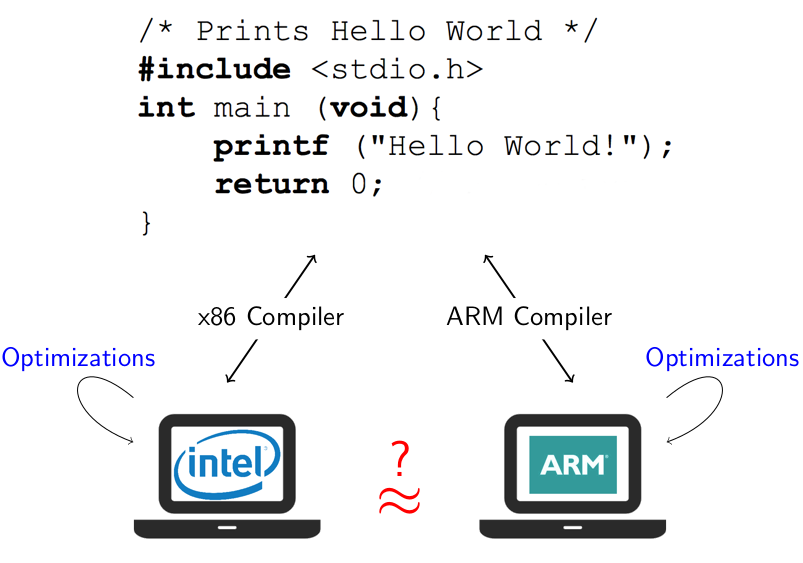
\includegraphics[height=0.4\textheight,keepaspectratio]{img/the-problem.png}
  \caption{The illustration of the portability problem~\cite{Porthos17slides}}
  \end{figure}
}
\end{minipage}
%
\begin{minipage}{.5\textwidth}
\only<2->{
  \begin{itemize}
    \begin{definition}[Portability~\cite{Porthos17a}]
    %SAY: Let $\textit{cons}_{\mathcal{M}}(P)$ be a function that calculates the set of executions of the program $P$ that are consistent under the memory model $\mathcal{M}$
    %Let $\mathcal{M_S}$, $\mathcal{M_T}$ be two weak memory models.
    The program $P$ is portable from the source memory model $\mathcal{M_S}$ to the target one $\mathcal{M_T}$ if
    $\textit{cons}_{\mathcal{M_T}}(P) \subseteq \textit{cons}_{\mathcal{M_S}}(P)$
    \end{definition}
    \item Portability as an SMT-based bounded reachability problem: \\
    $\phi = $\only<3>\yellowemph{$\phi_{CF}$}$\land $\only<3>\yellowemph{$\phi_{DF}$}$\land \phi_{\mathcal{M_T}} \land \phi_{\lnot\mathcal{M_S}}$
    \item $\texttt{SAT}(\phi) \Longrightarrow $ portability bug
  \end{itemize}
}
\end{minipage}
\end{frame}



\begin{frame}{\tool{PorthosC}: Architecture}{Main components}
\vspace{-30pt}
\begin{minipage}{.49\textwidth}
\begin{itemize}
\item The enhanced version of \tool{Porthos}, that is able to analyse C programs, has got a new name \textit{PorthosC}.
\end{itemize}
\hfill
\end{minipage}
%
\begin{minipage}{.5\textwidth}
\only<1>{\begin{figure}
  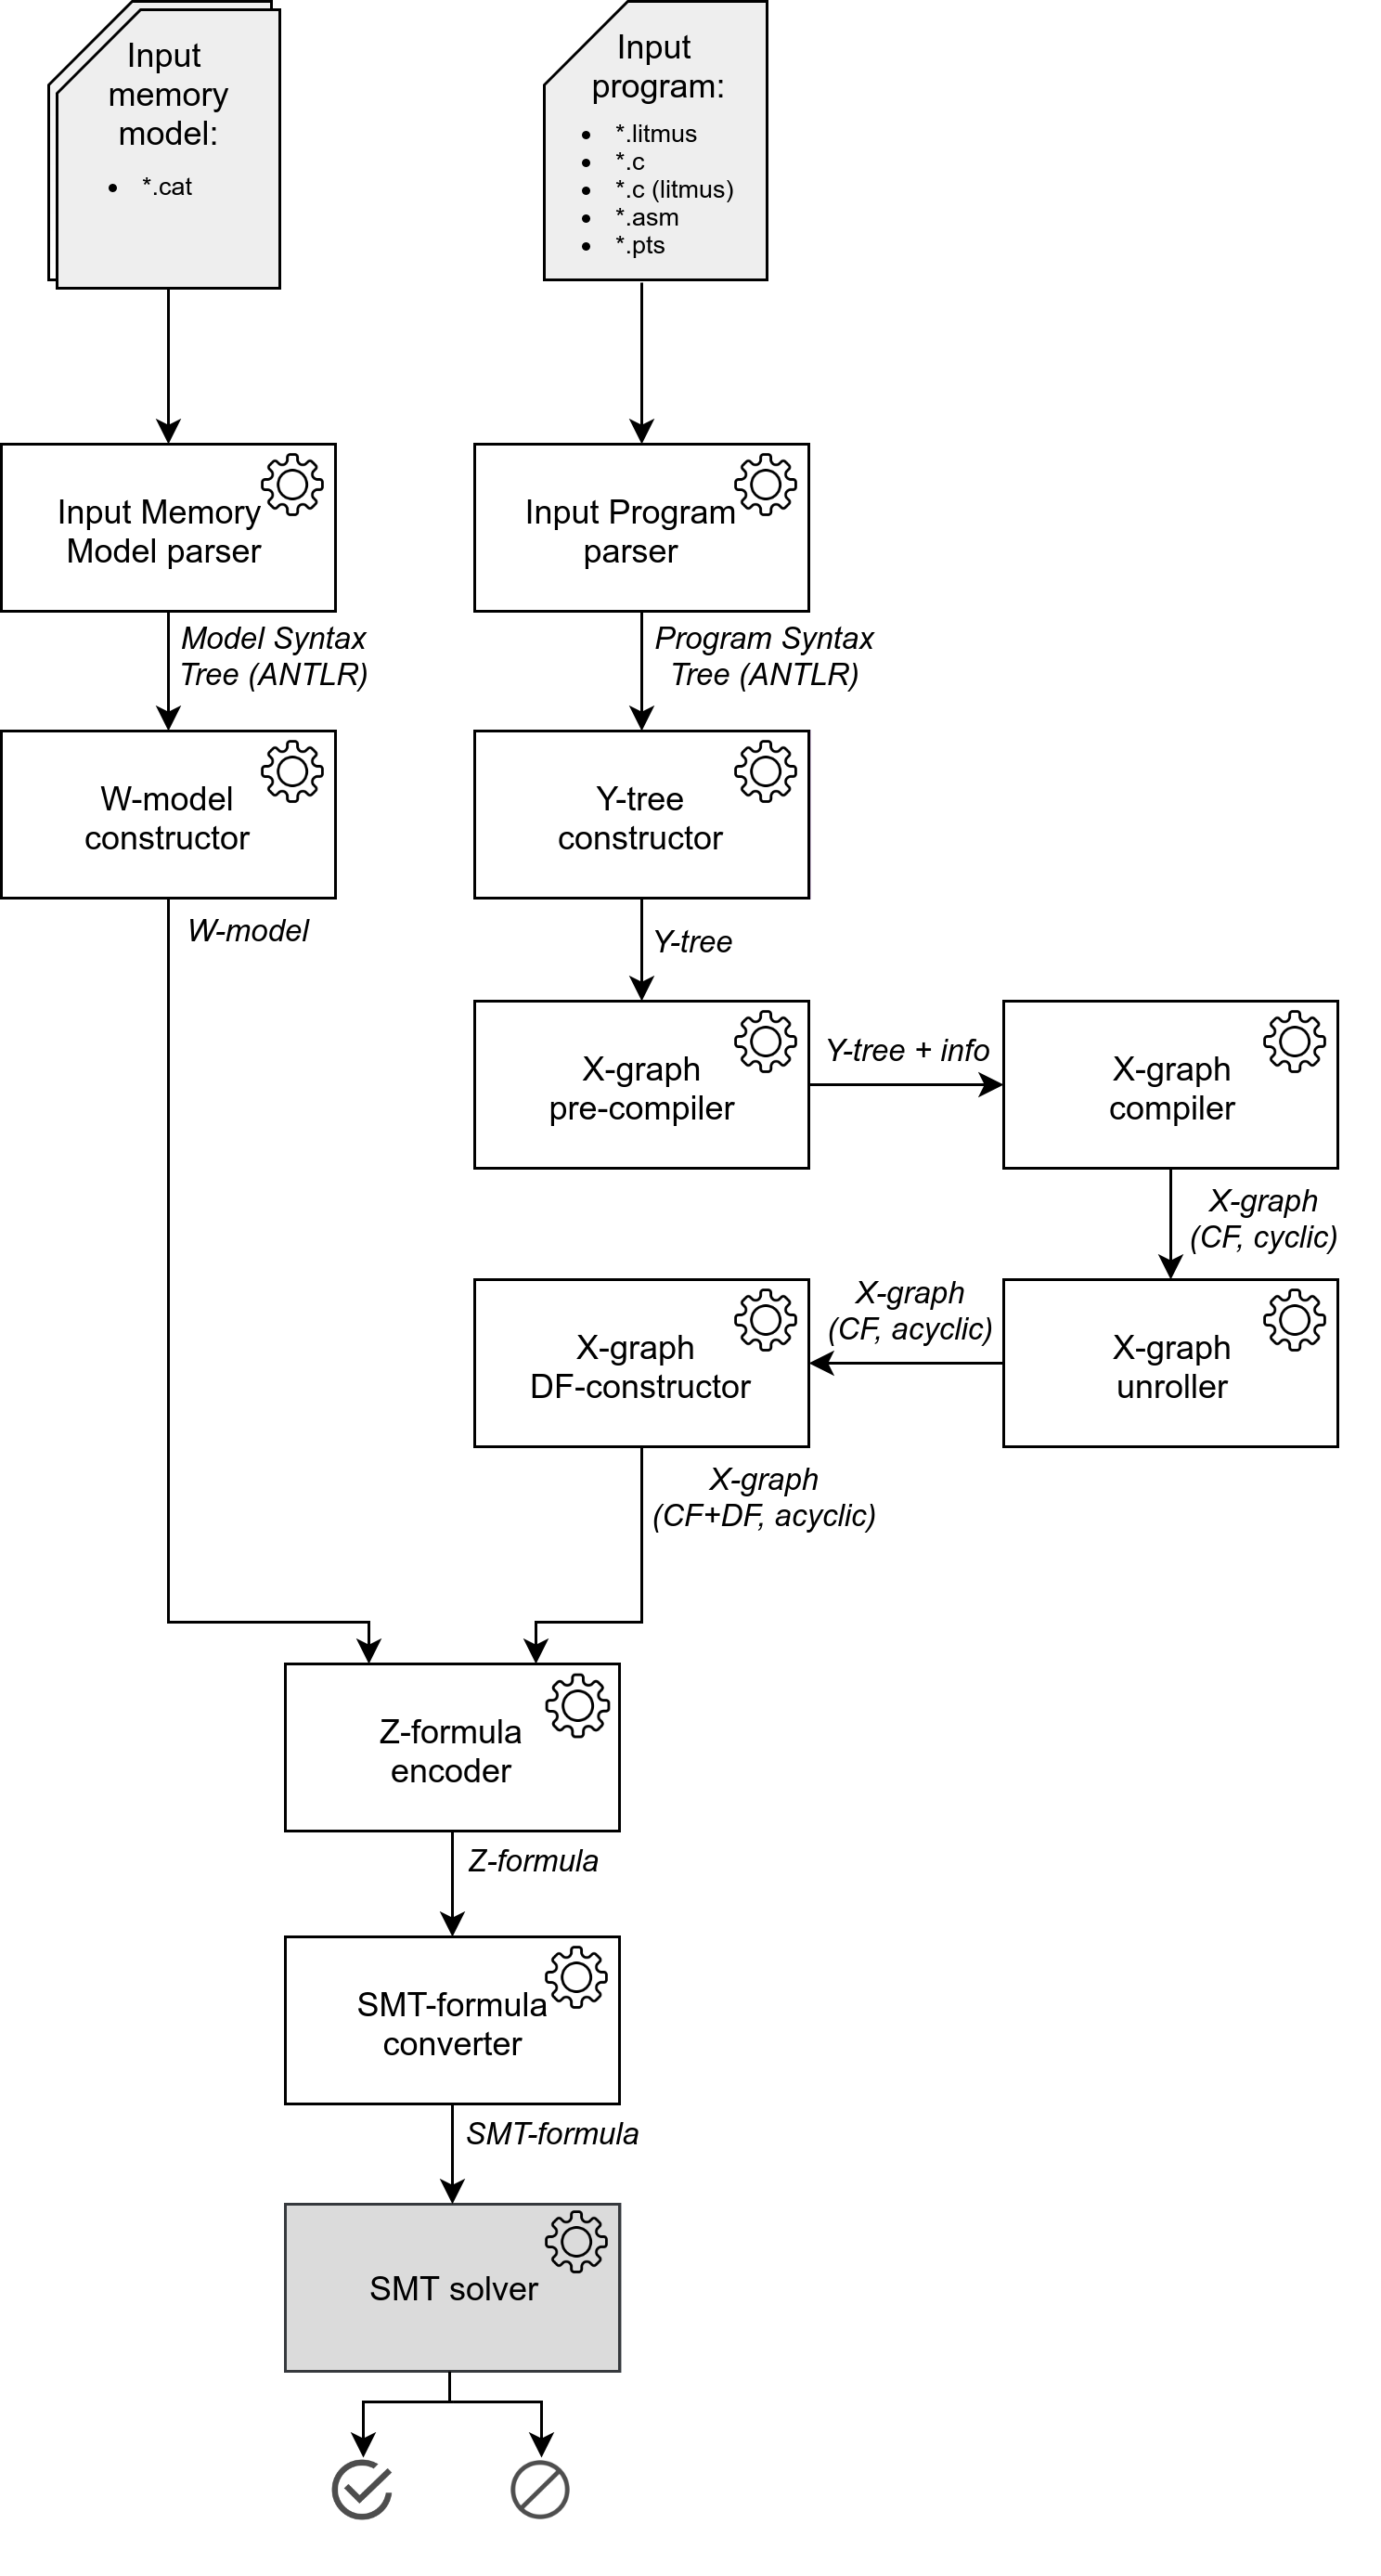
\includegraphics[height=.98\textheight,keepaspectratio]{img/arch/general_arch-no_numbering.png}
\end{figure}}
\only<2>{\begin{figure}
  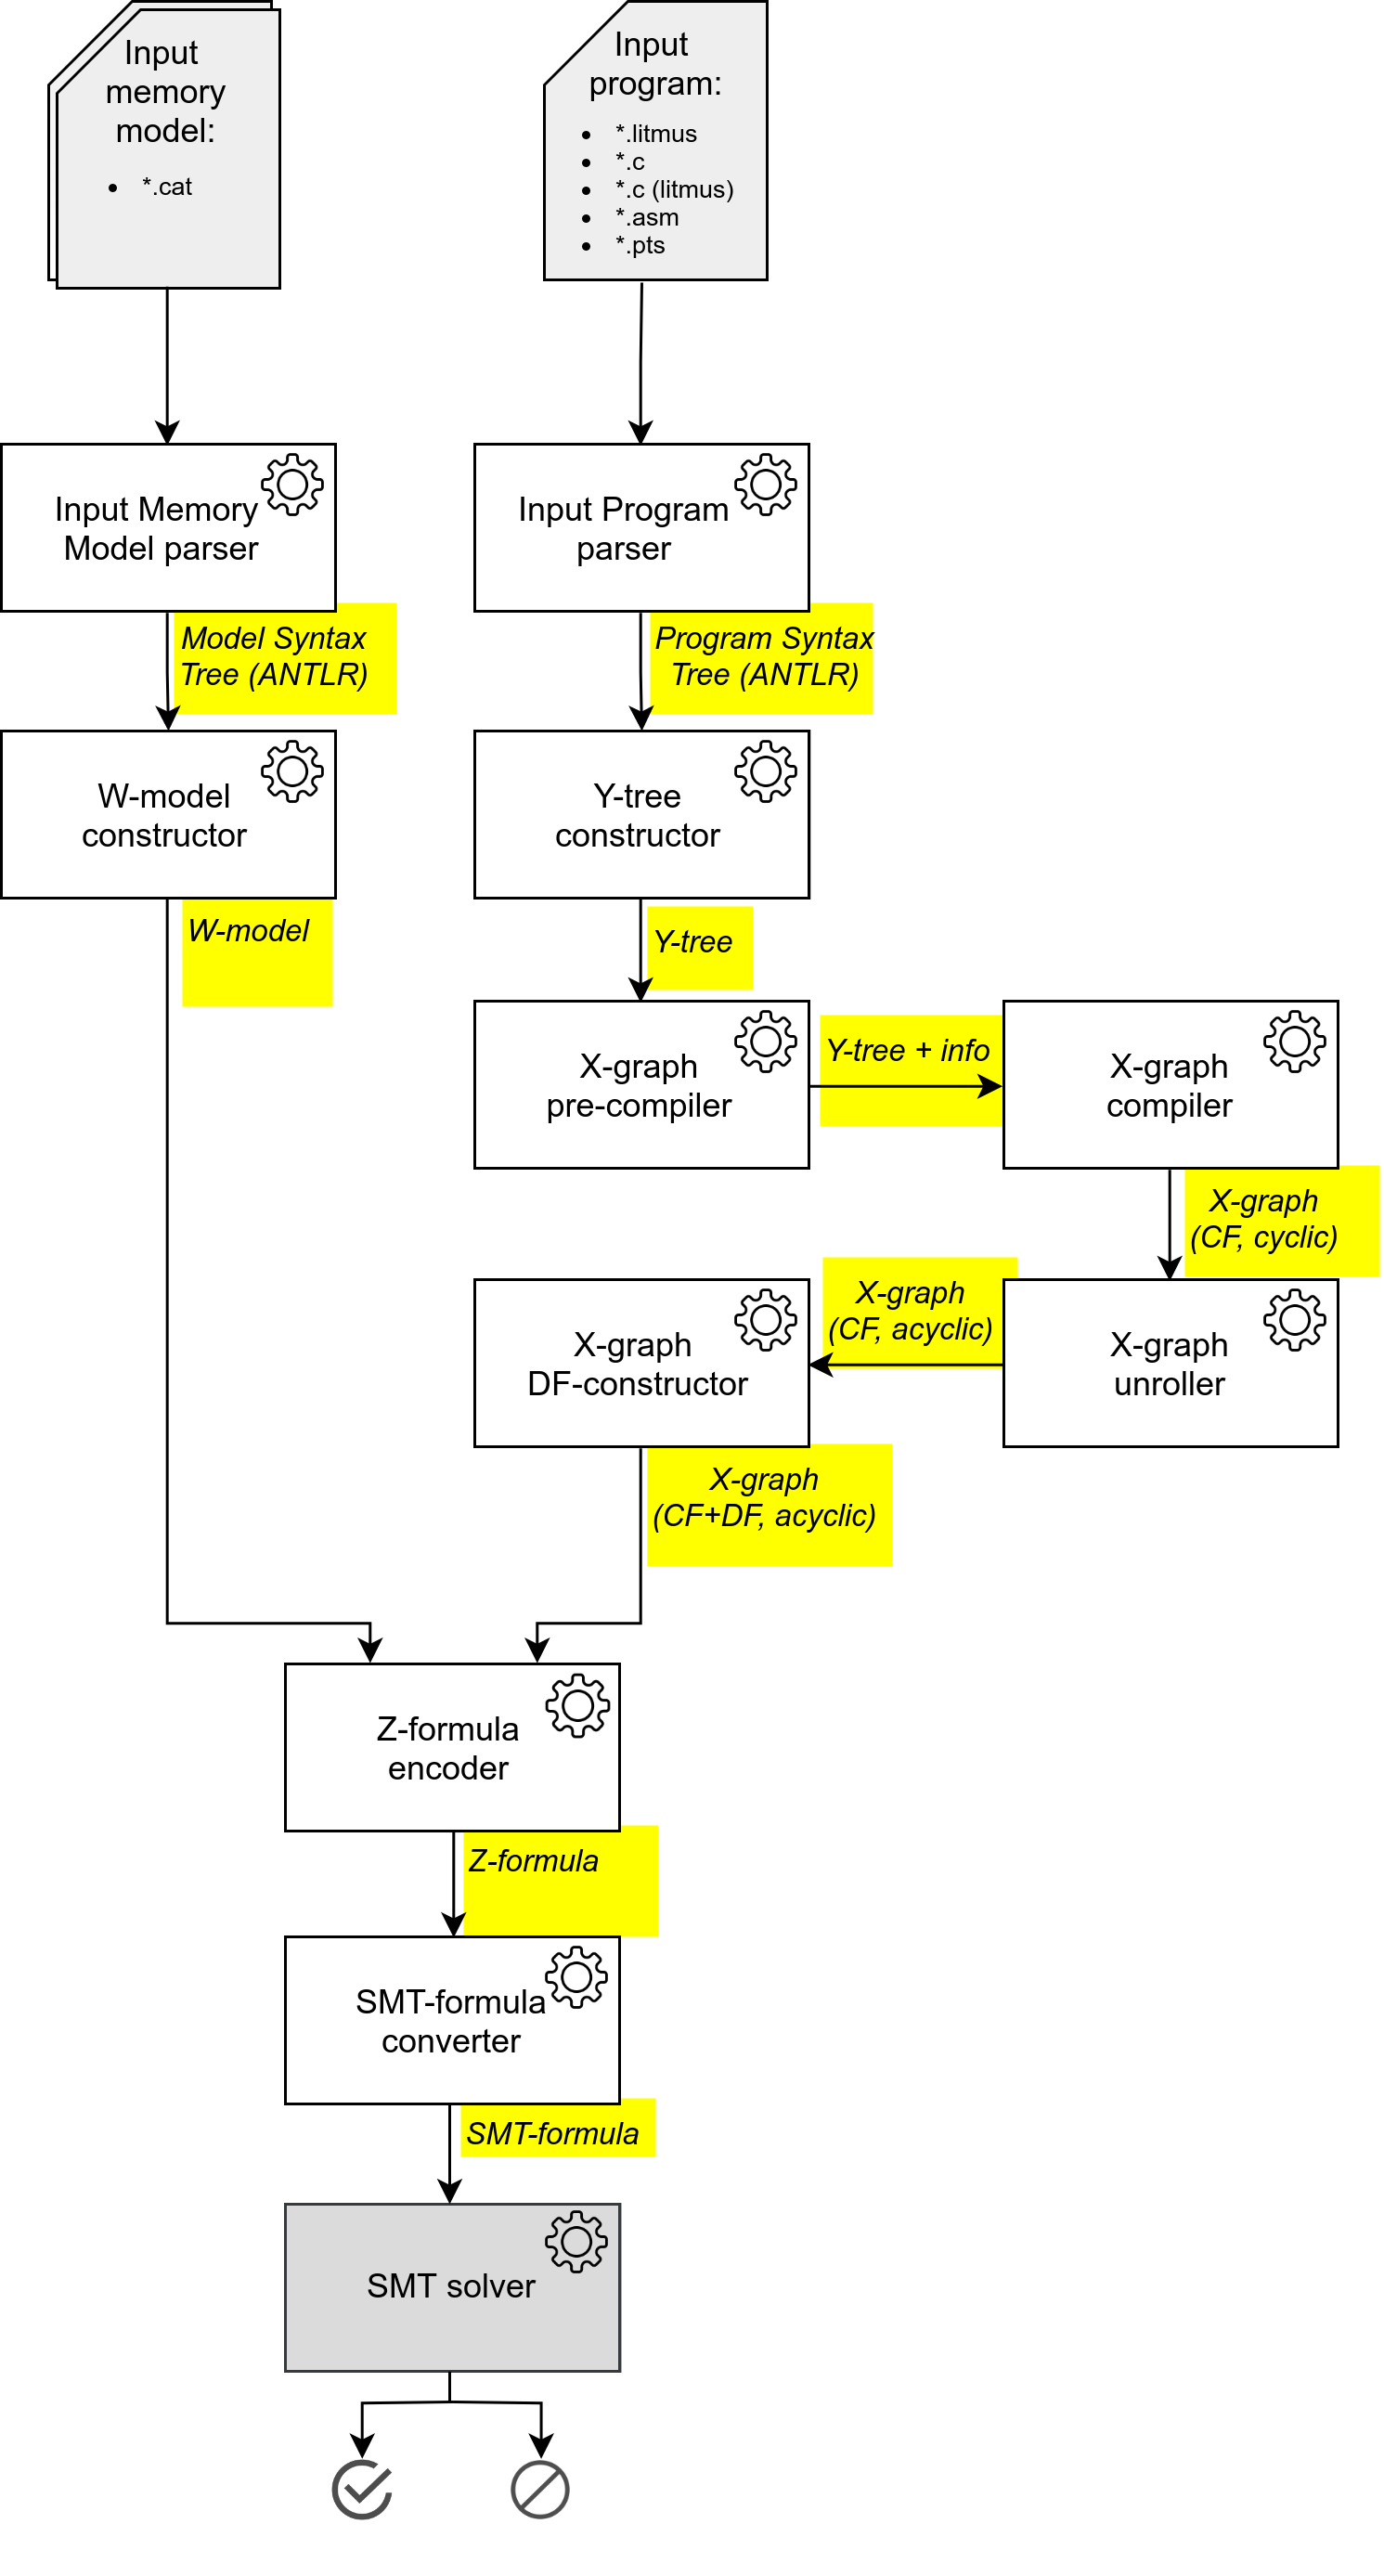
\includegraphics[height=.98\textheight,keepaspectratio]{img/arch/general_arch-no_numbering-labels.png}
\end{figure}}
\only<3>{\begin{figure}
  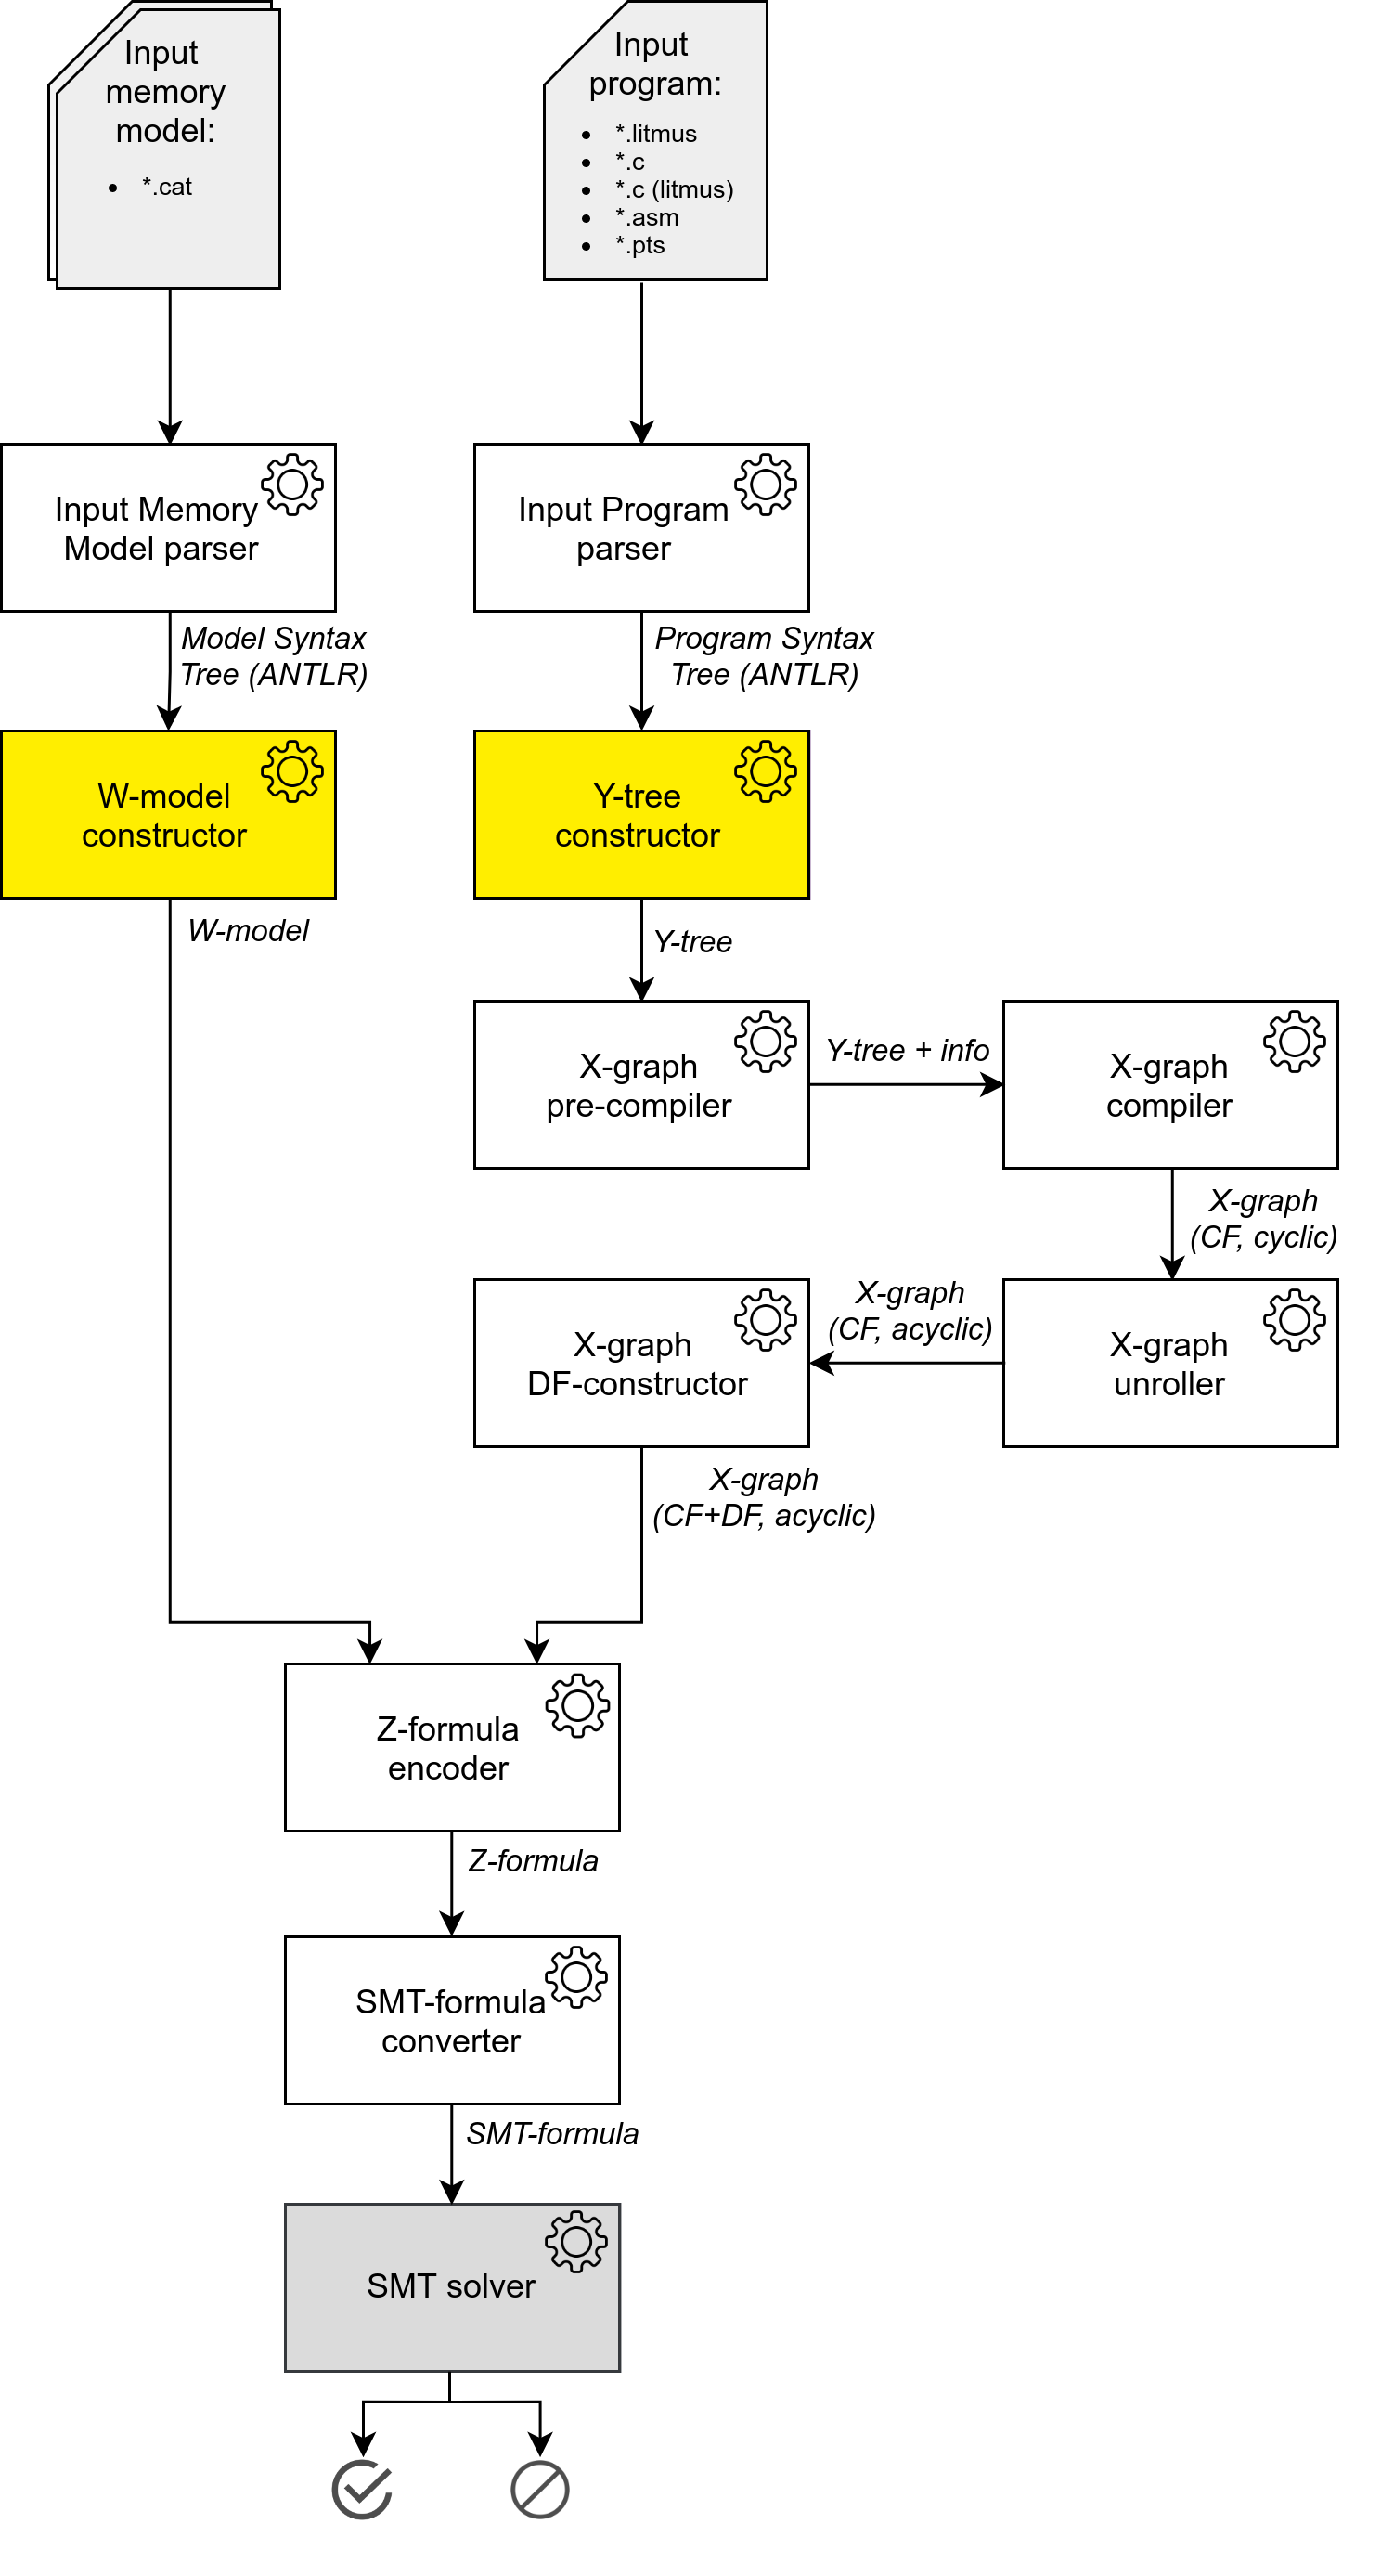
\includegraphics[height=.98\textheight,keepaspectratio]{img/arch/general_arch-no_numbering-visitors.png}
\end{figure}}
\only<4>{\begin{figure}
  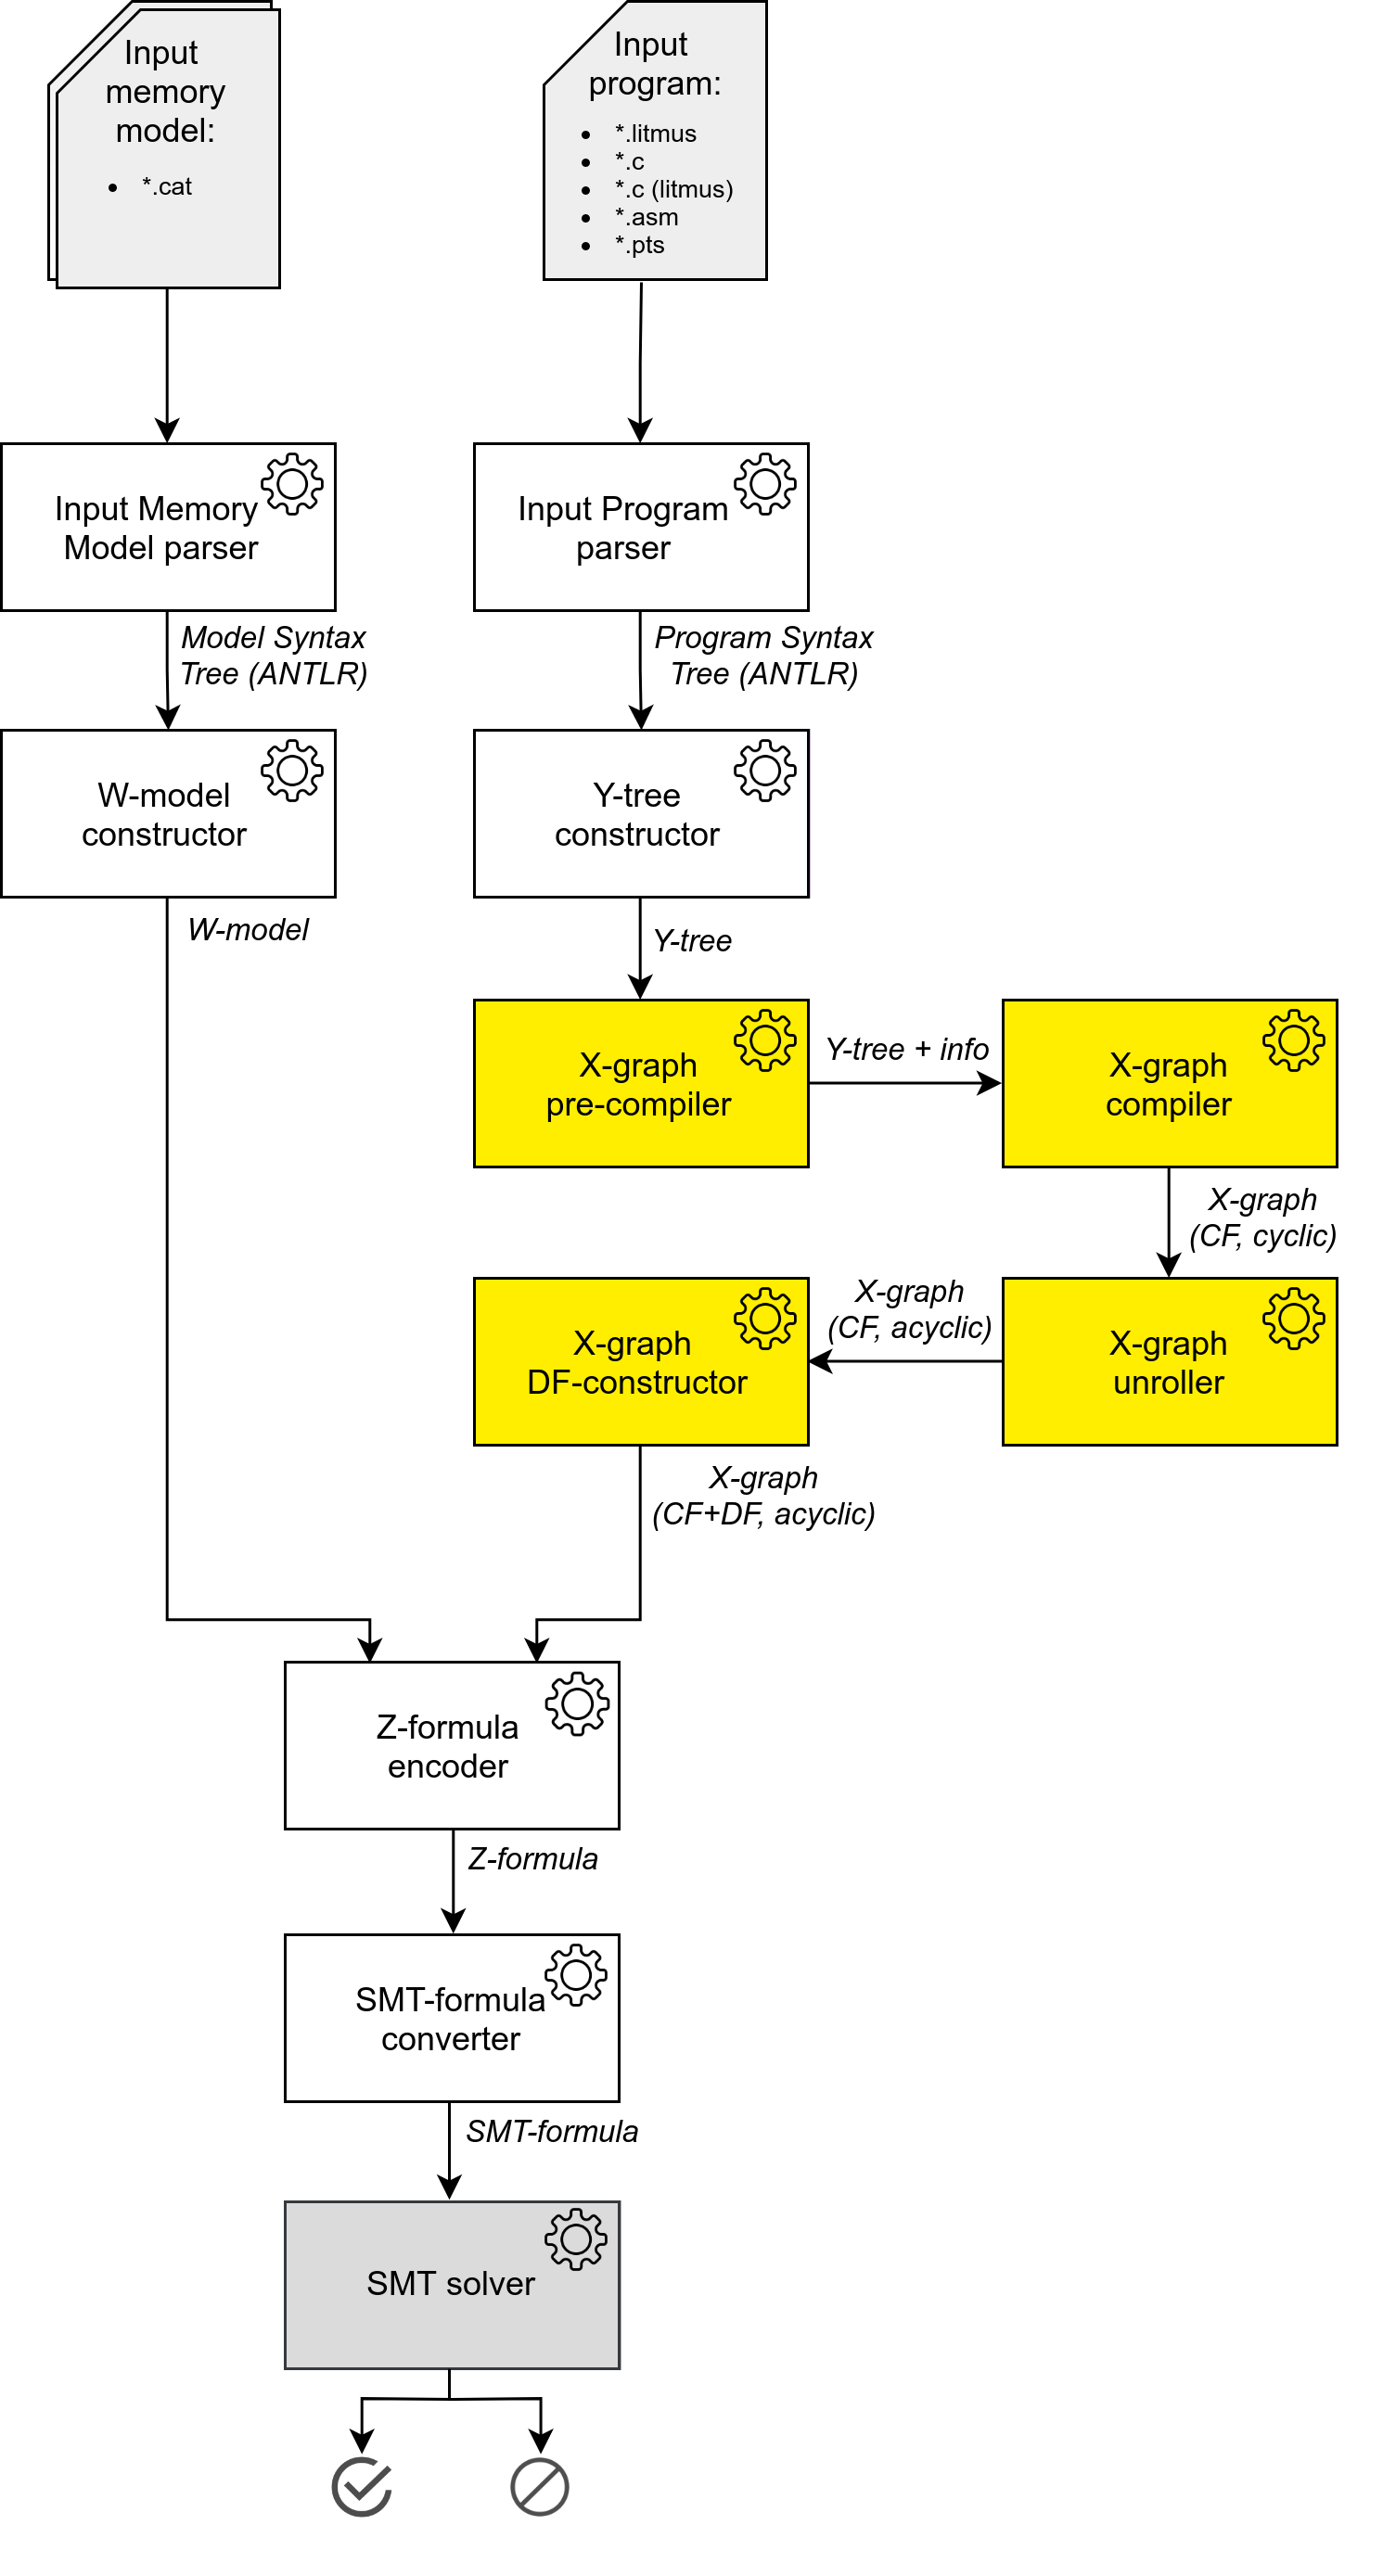
\includegraphics[height=.98\textheight,keepaspectratio]{img/arch/general_arch-no_numbering-compiler.png}
\end{figure}}
\only<5>{\begin{figure}
  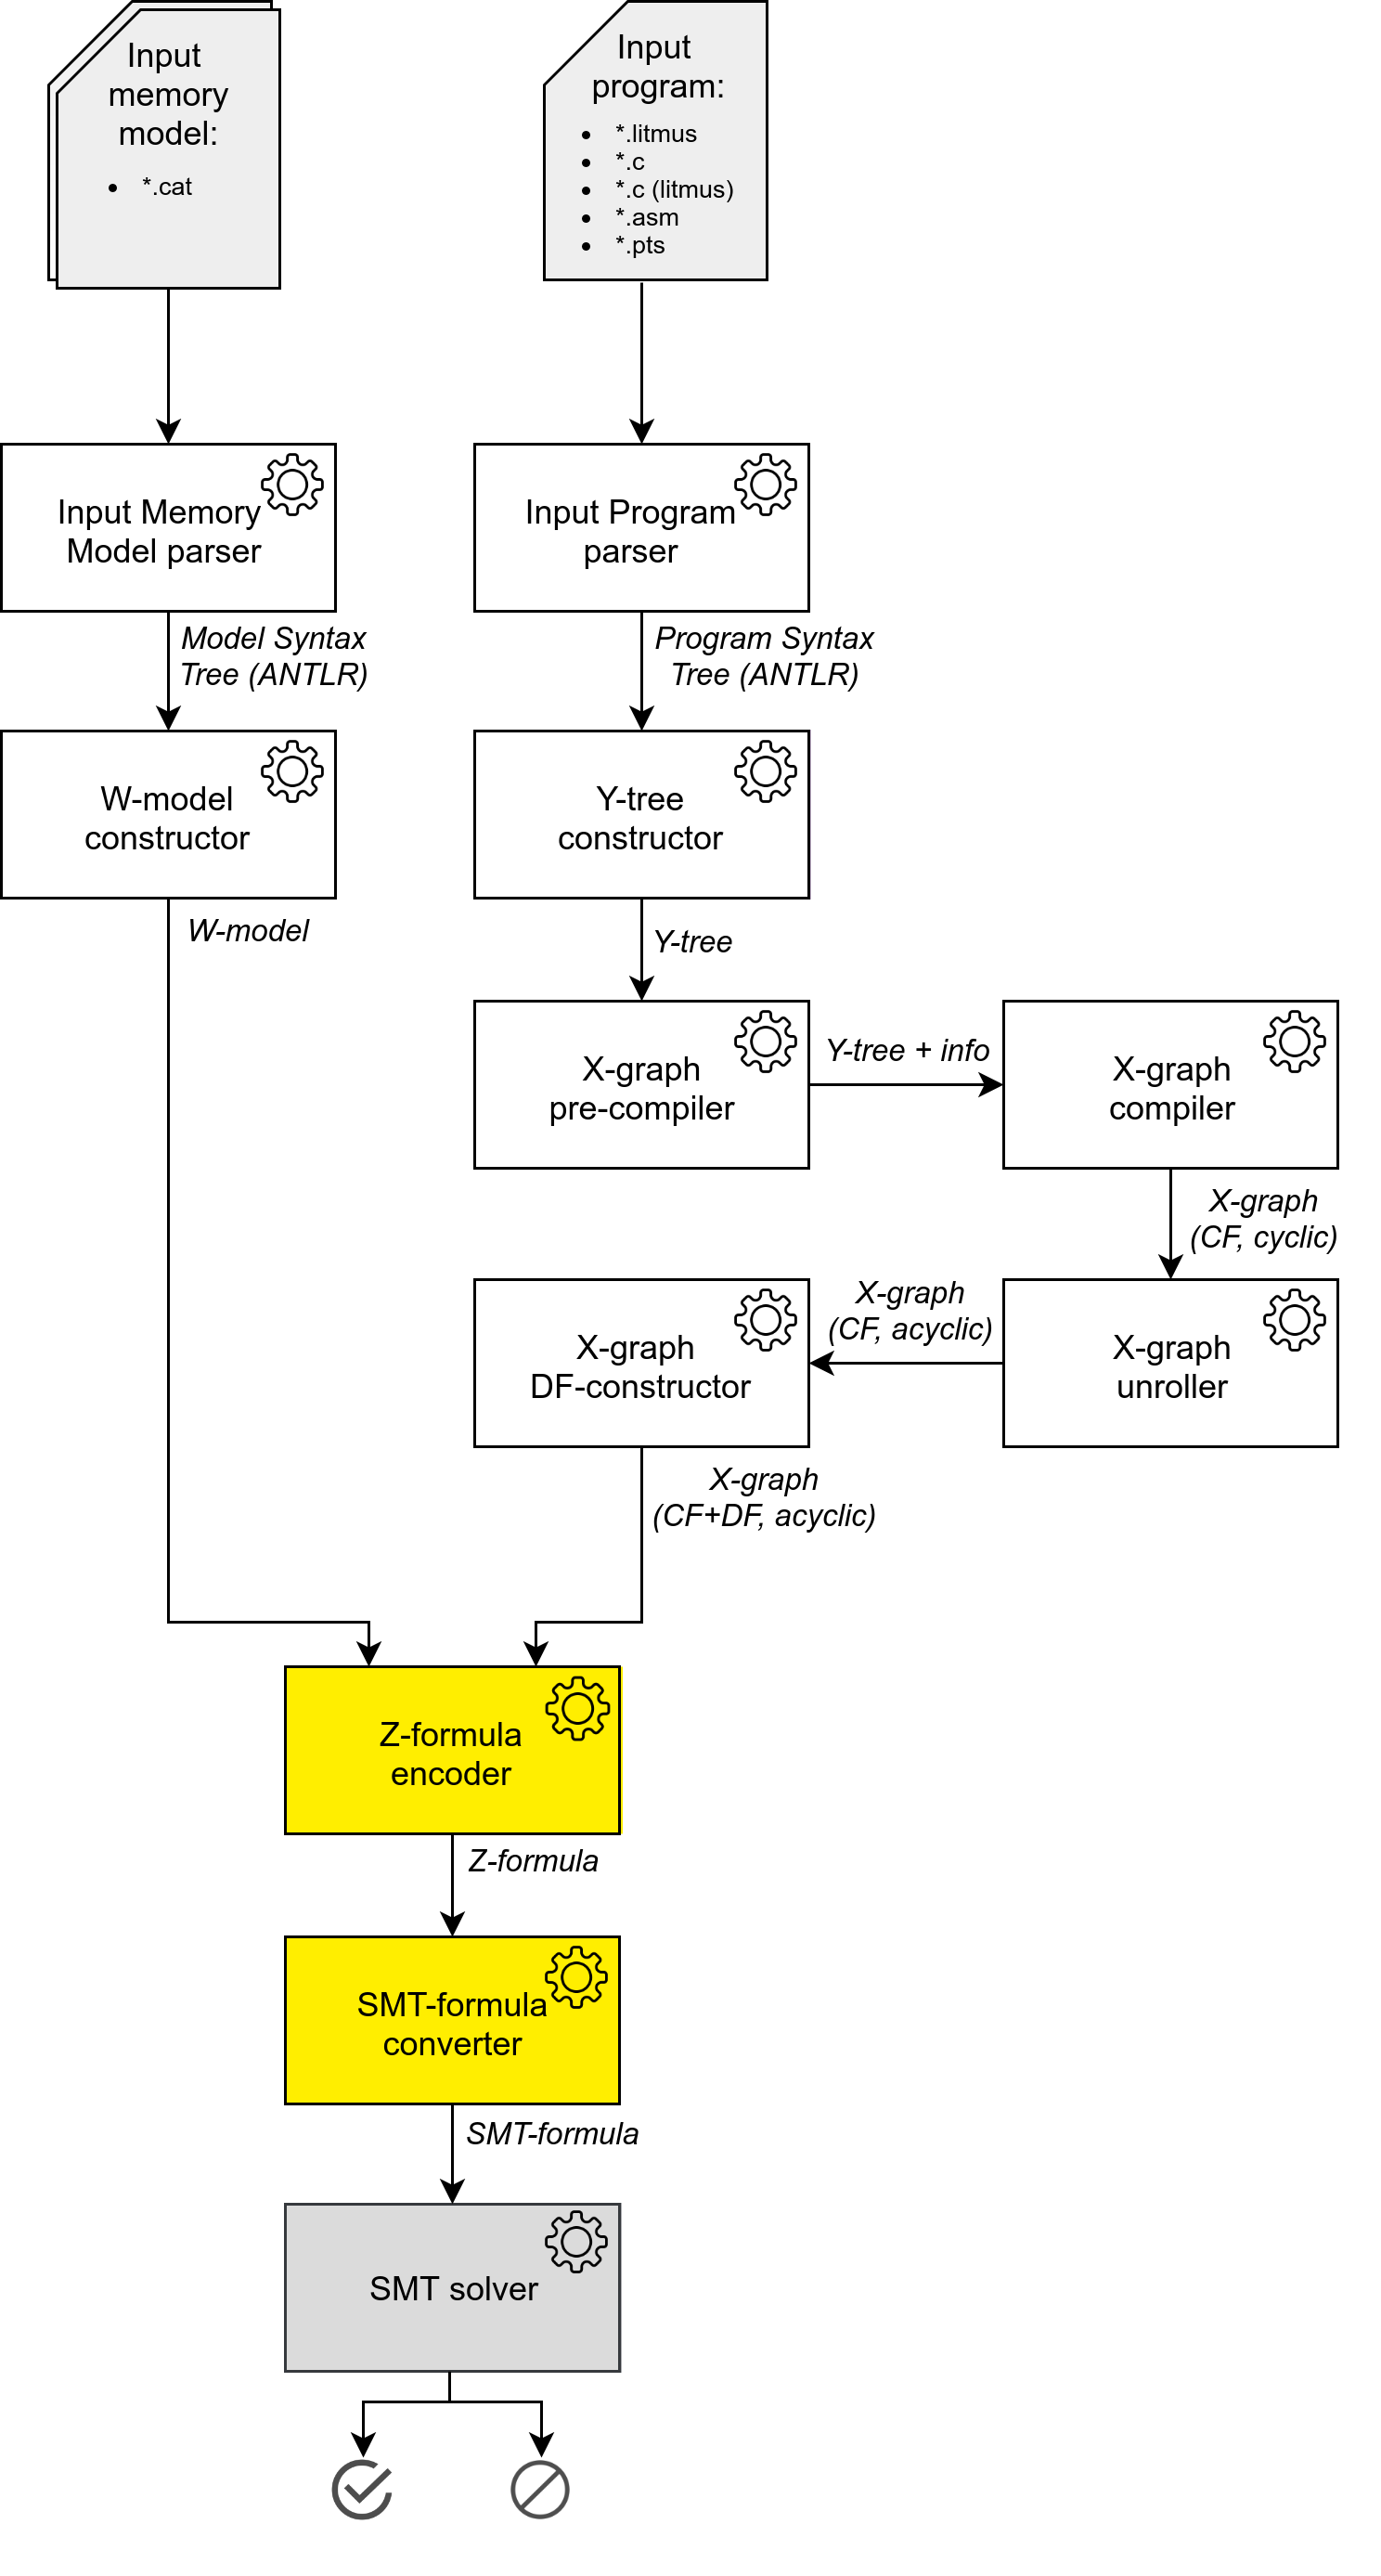
\includegraphics[height=.98\textheight,keepaspectratio]{img/arch/general_arch-no_numbering-smt.png}
\end{figure}}
\end{minipage}
\end{frame}



\begin{frame}{\tool{PorthosC}: Architecture}{Abstract interpretation module}
  \vspace{-40pt}
\begin{minipage}{.4\textwidth}
\begin{itemize}
\item The abstract interpretation module is an essential part of the compiler of C code into the event-flow graph representation (\texttt{X-graph}).
\end{itemize}
\hfill
\end{minipage}
%
\begin{minipage}{.5\textwidth}
\only<1>{\begin{figure}
  \scalebox{0.9}{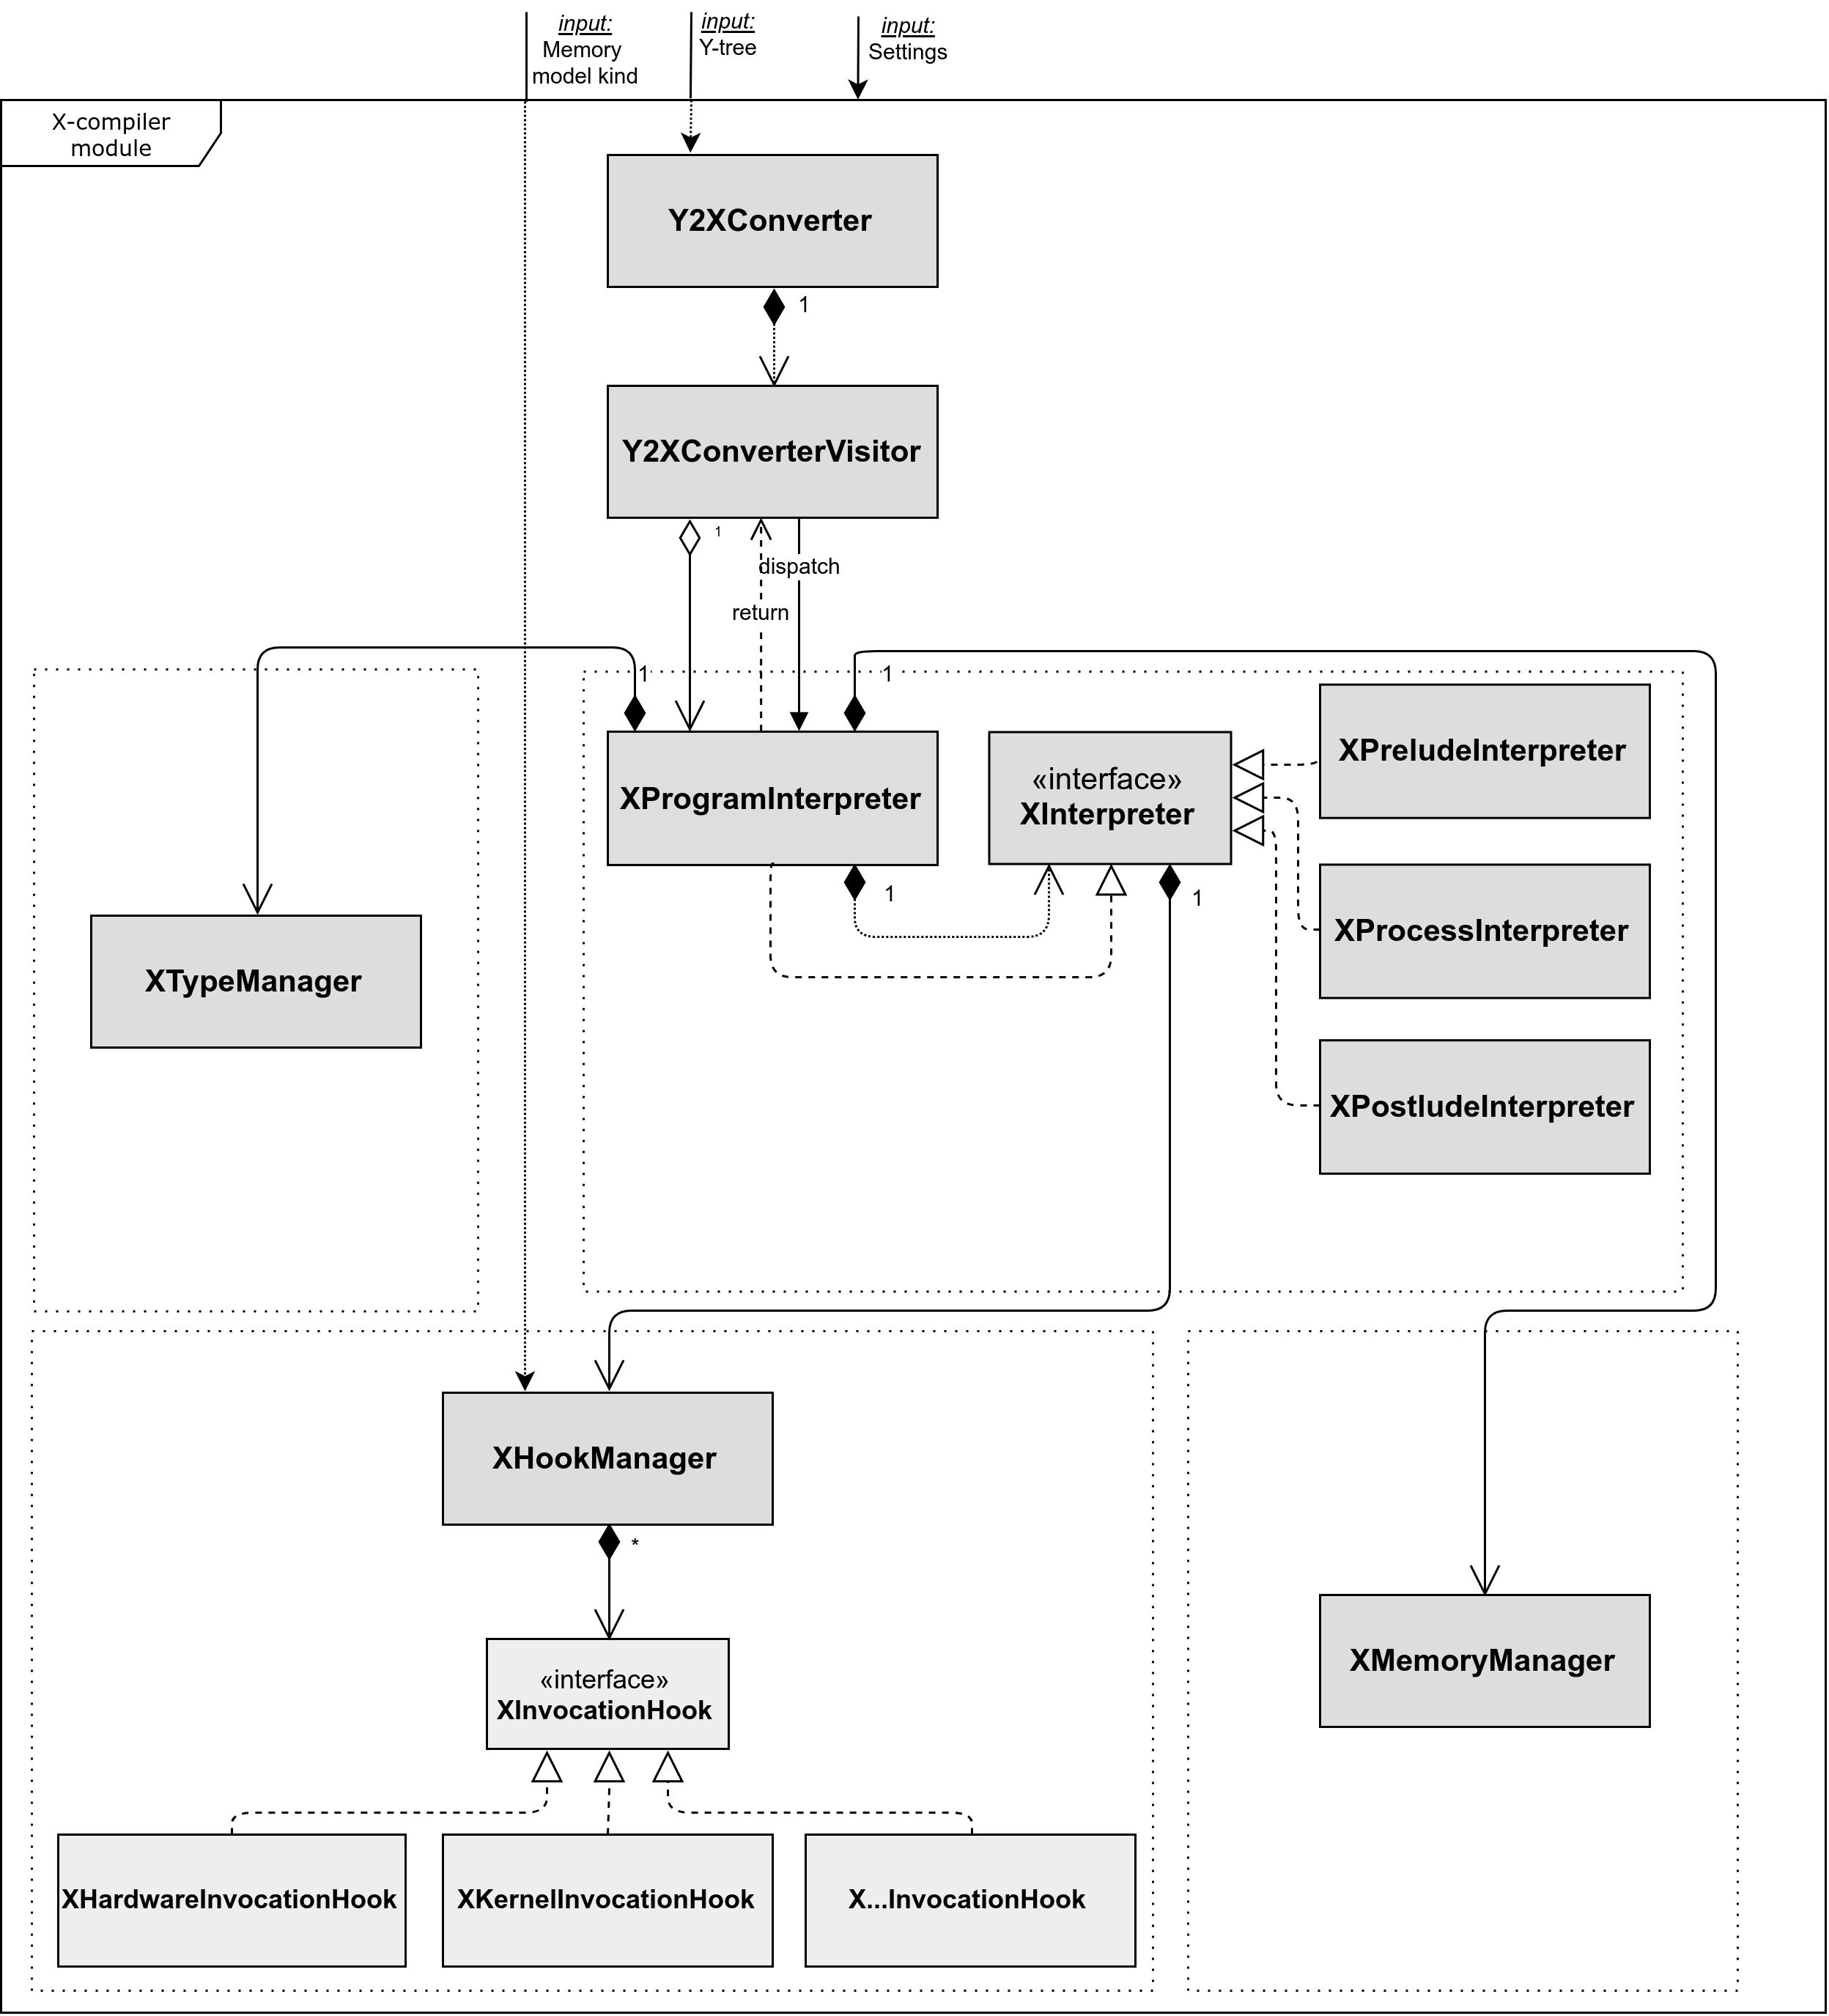
\includegraphics[height=.99\paperheight]{img/compiler/X-compiler.png}}
\end{figure}}
\only<2>{\begin{figure}
  \scalebox{0.9}{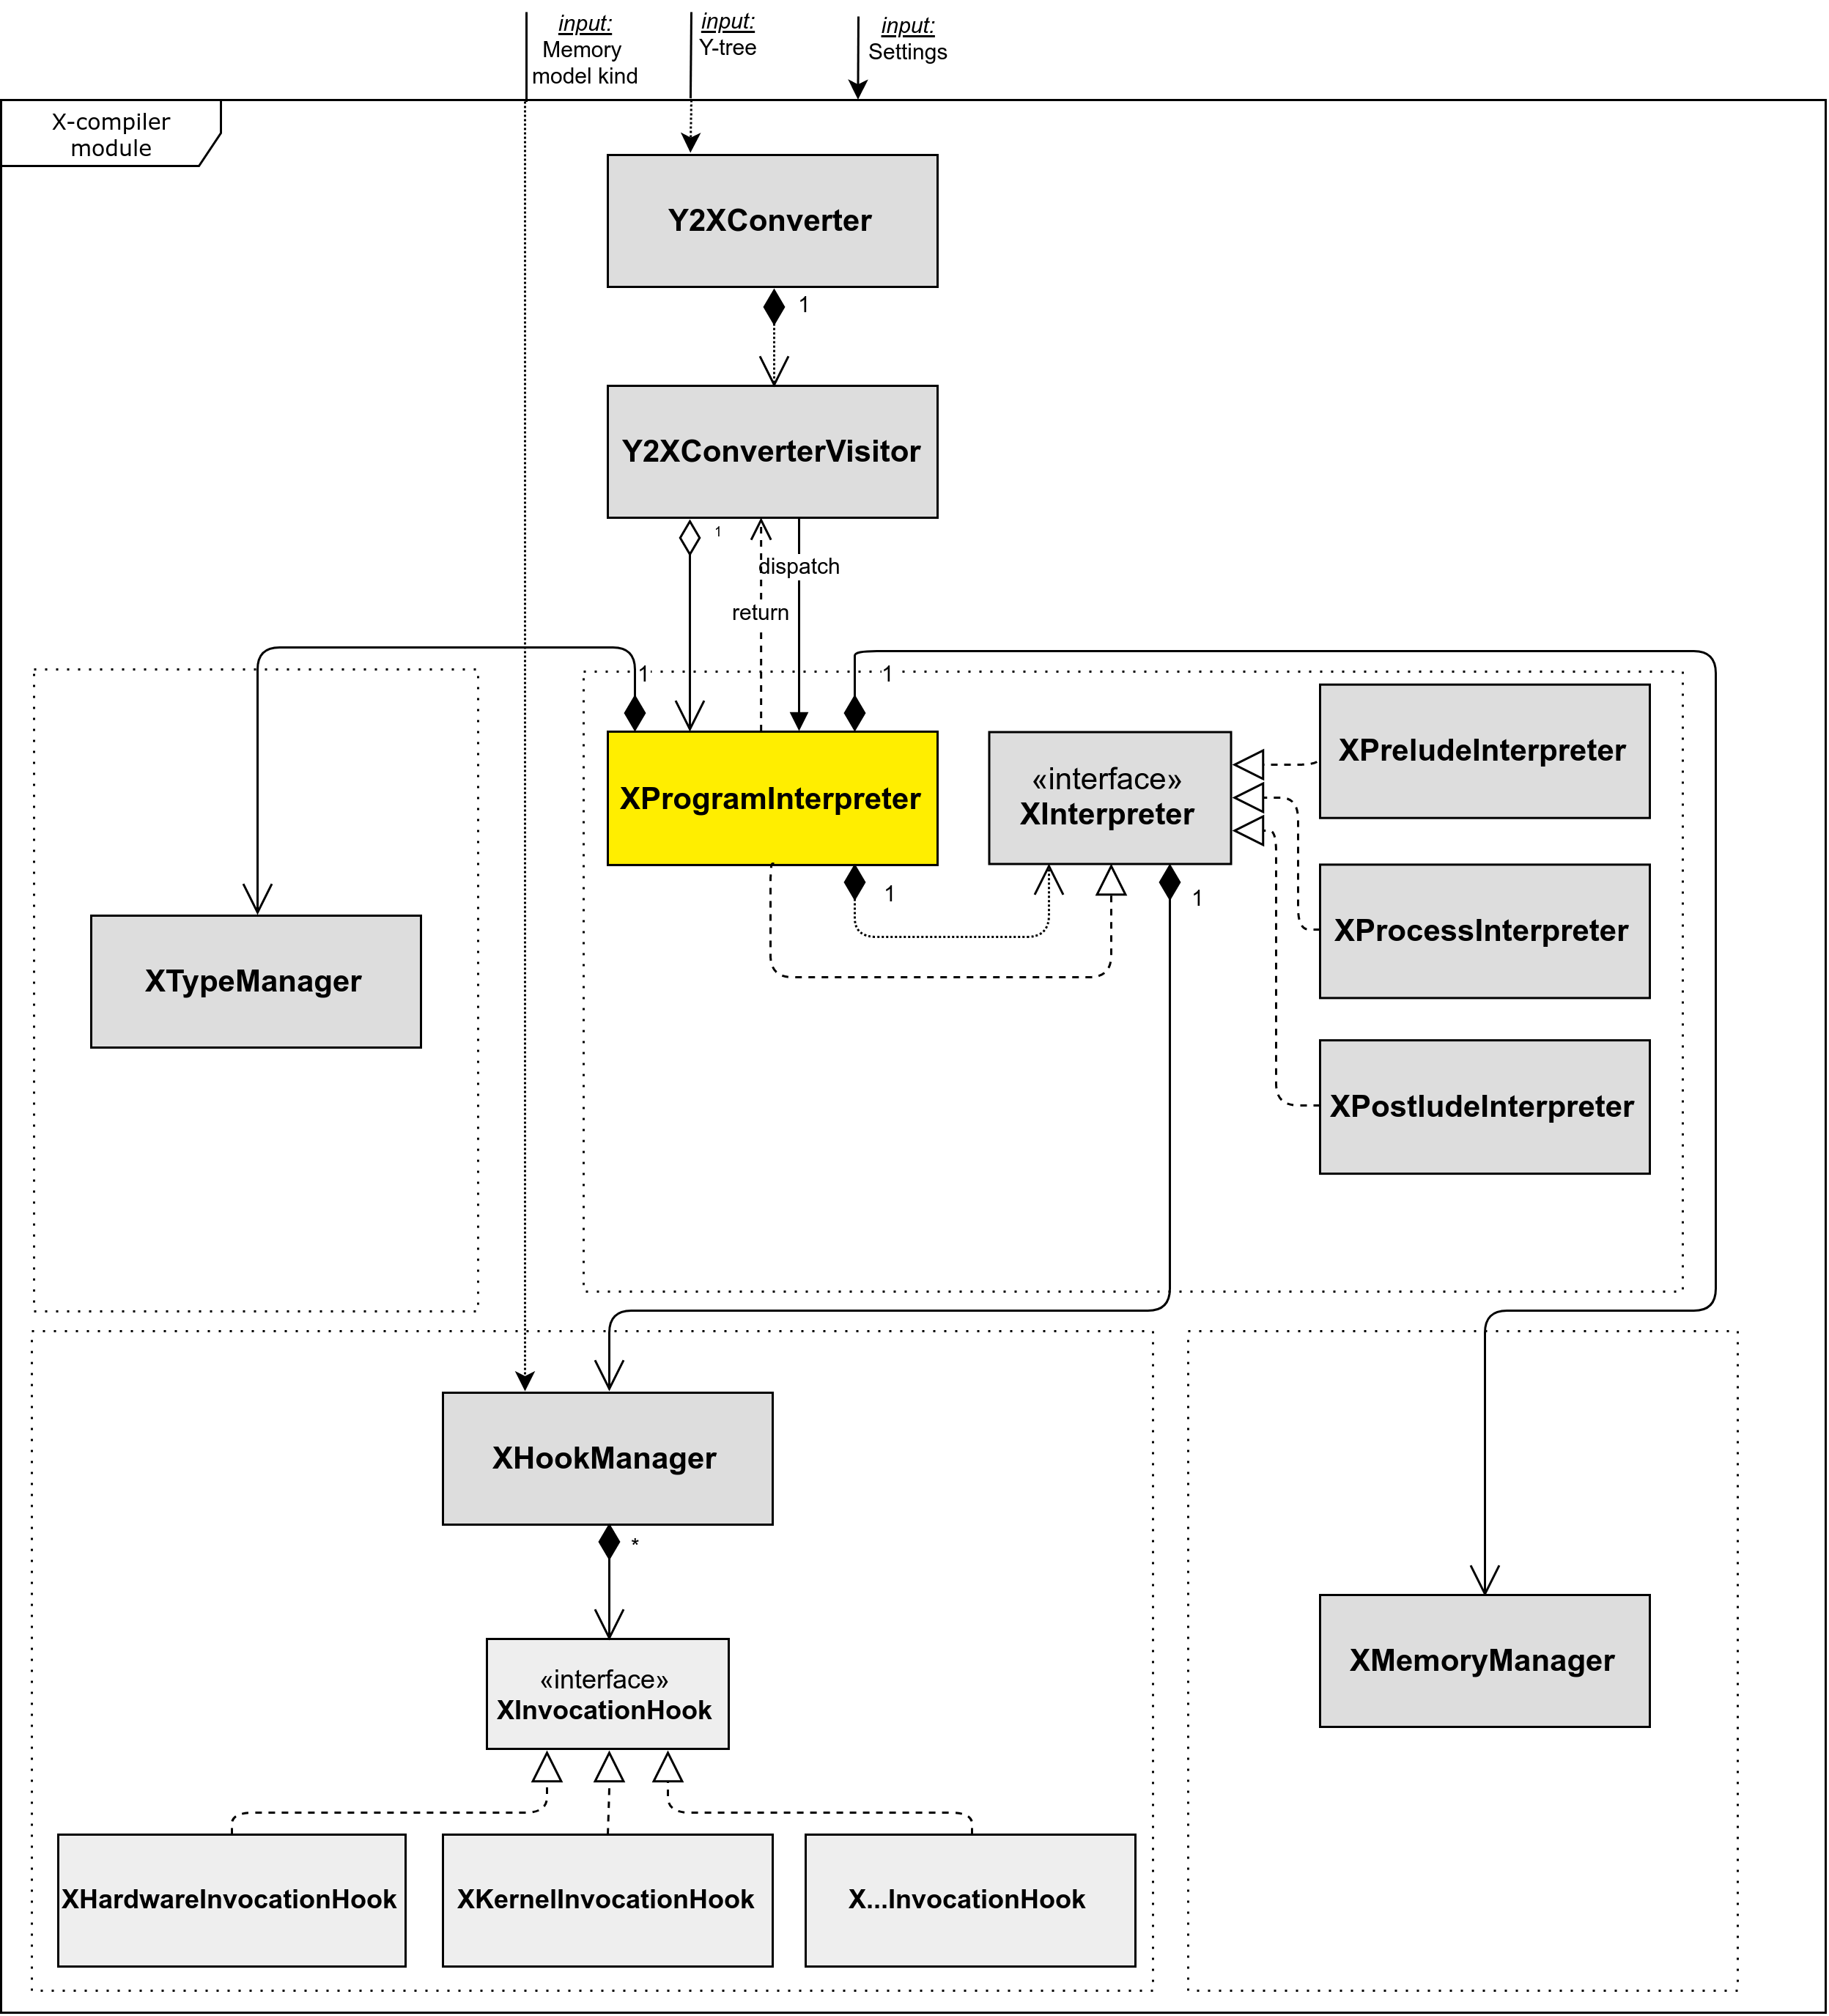
\includegraphics[height=.99\paperheight]{img/compiler/X-compiler-1.png}}
\end{figure}}
\only<3>{\begin{figure}
  \scalebox{0.9}{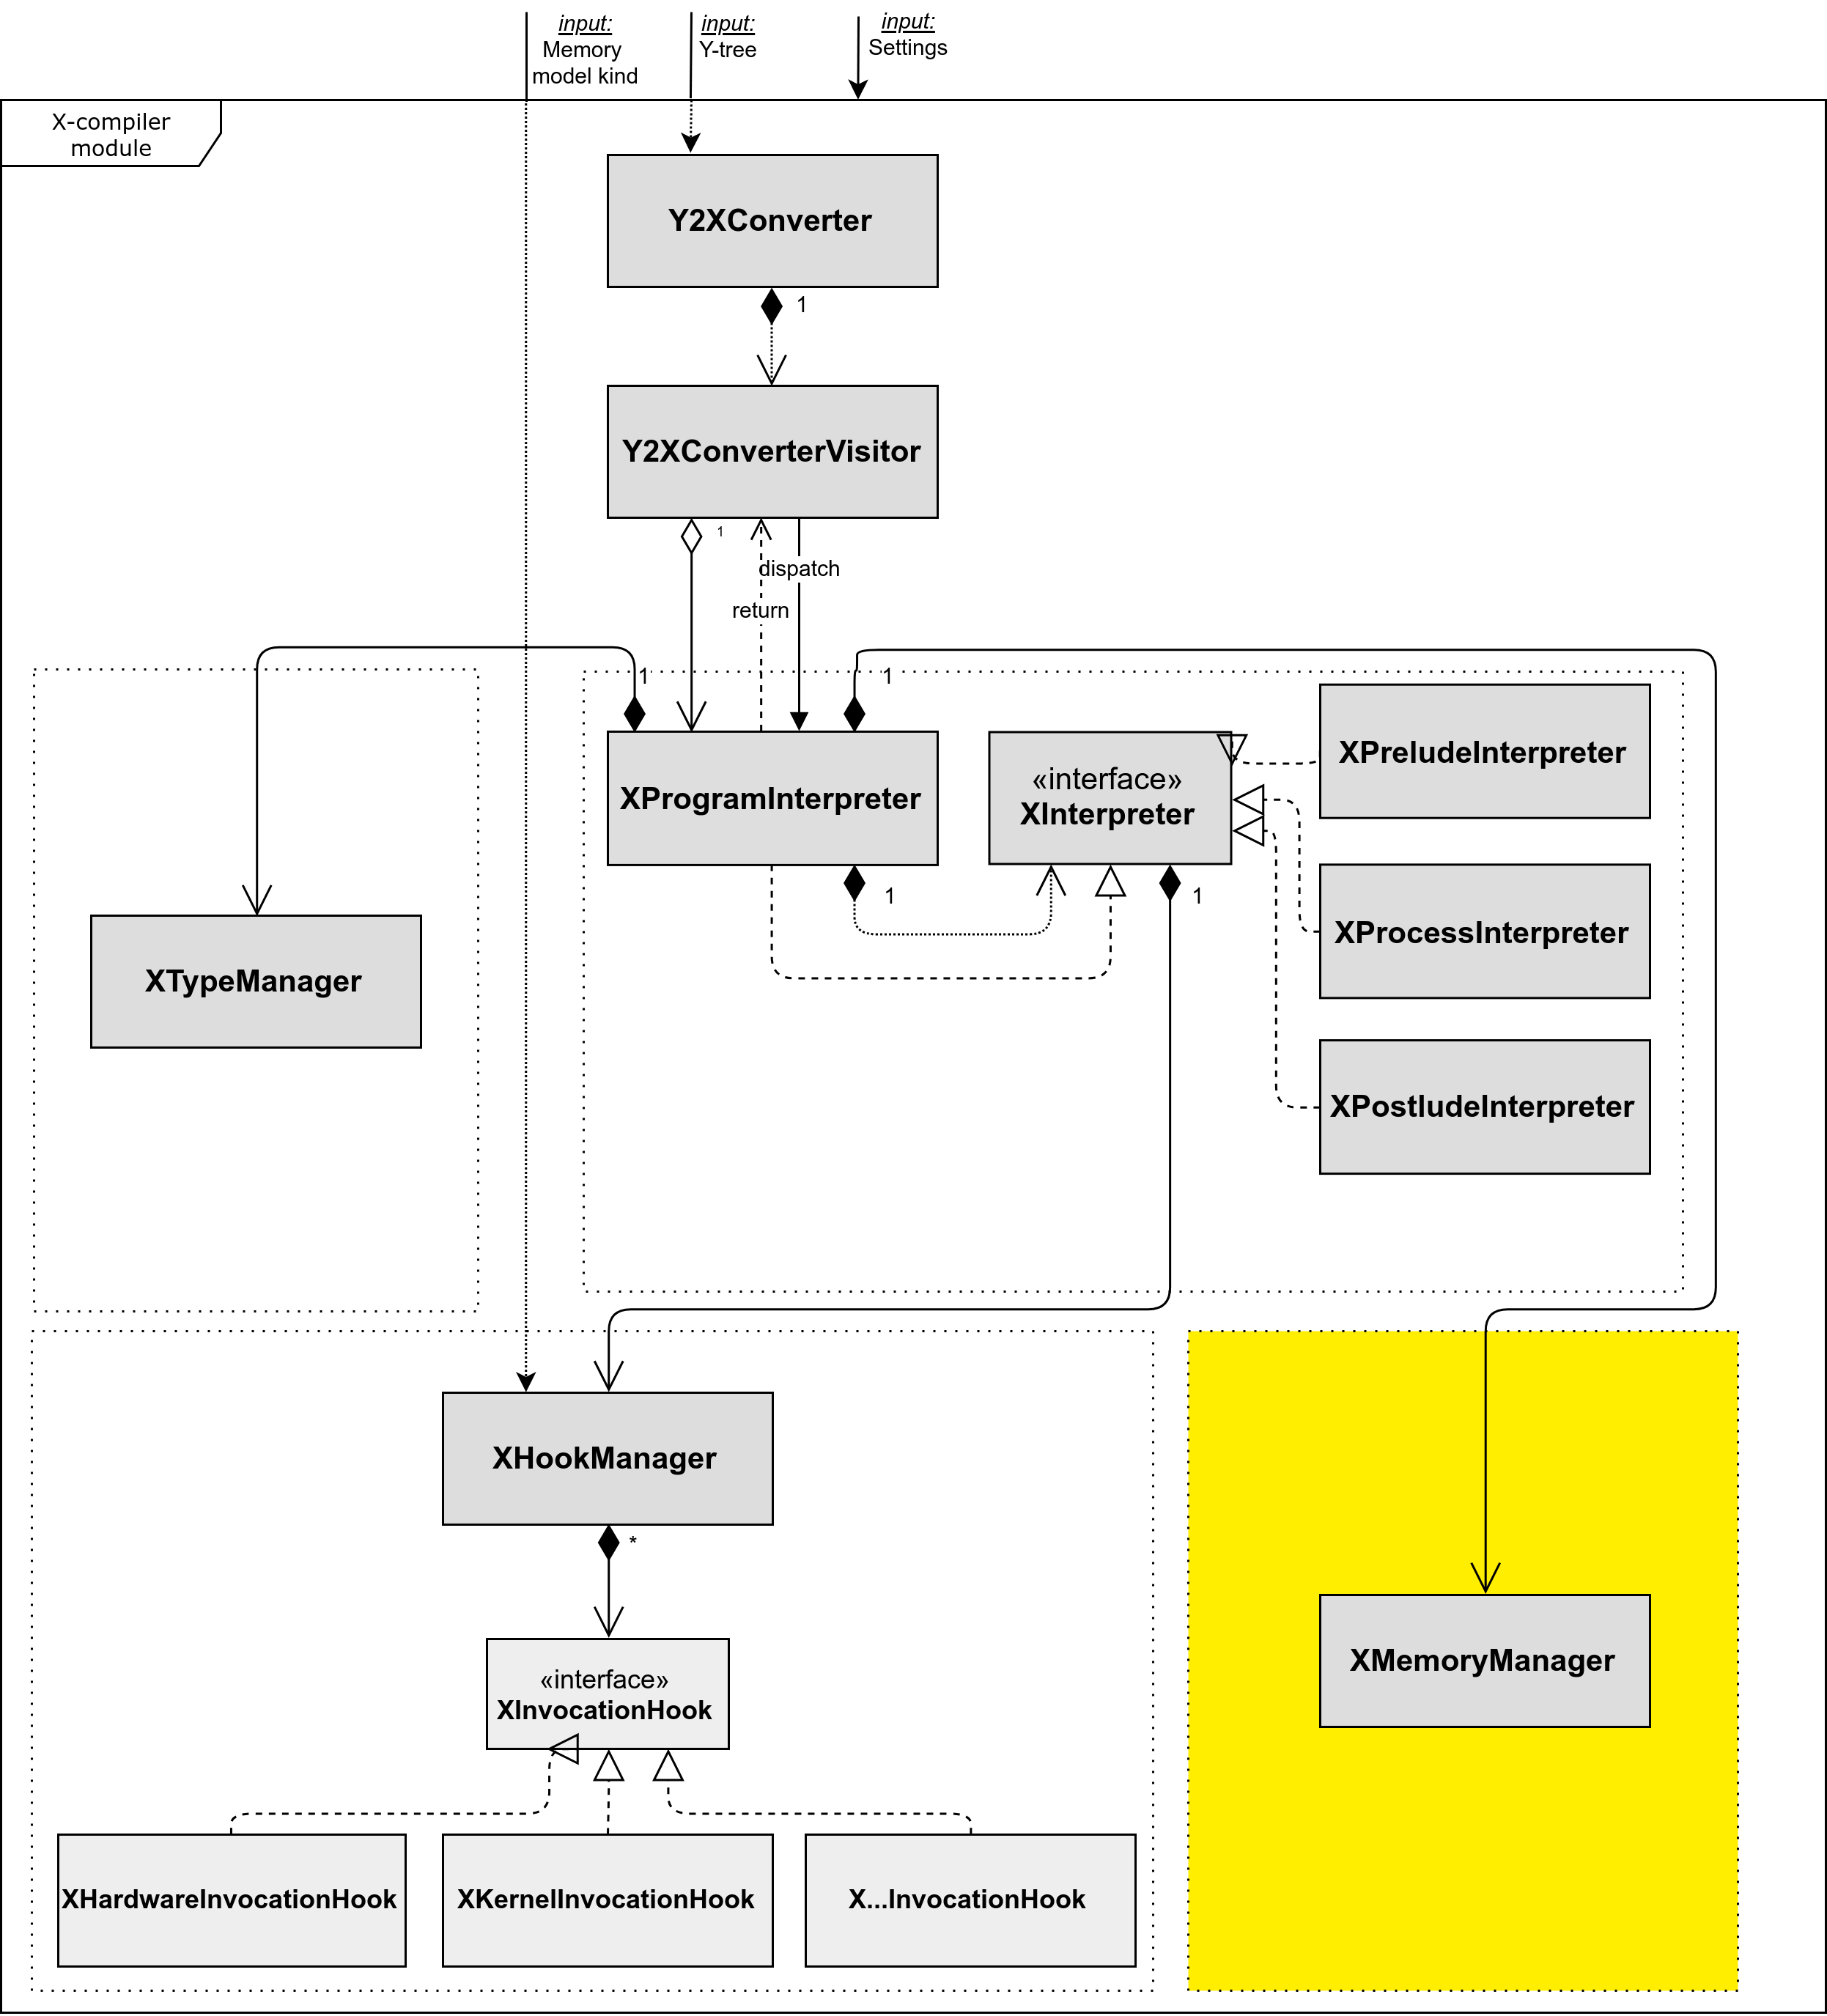
\includegraphics[height=.99\paperheight]{img/compiler/X-compiler-2.png}}
\end{figure}}
\only<4>{\begin{figure}
  \scalebox{0.9}{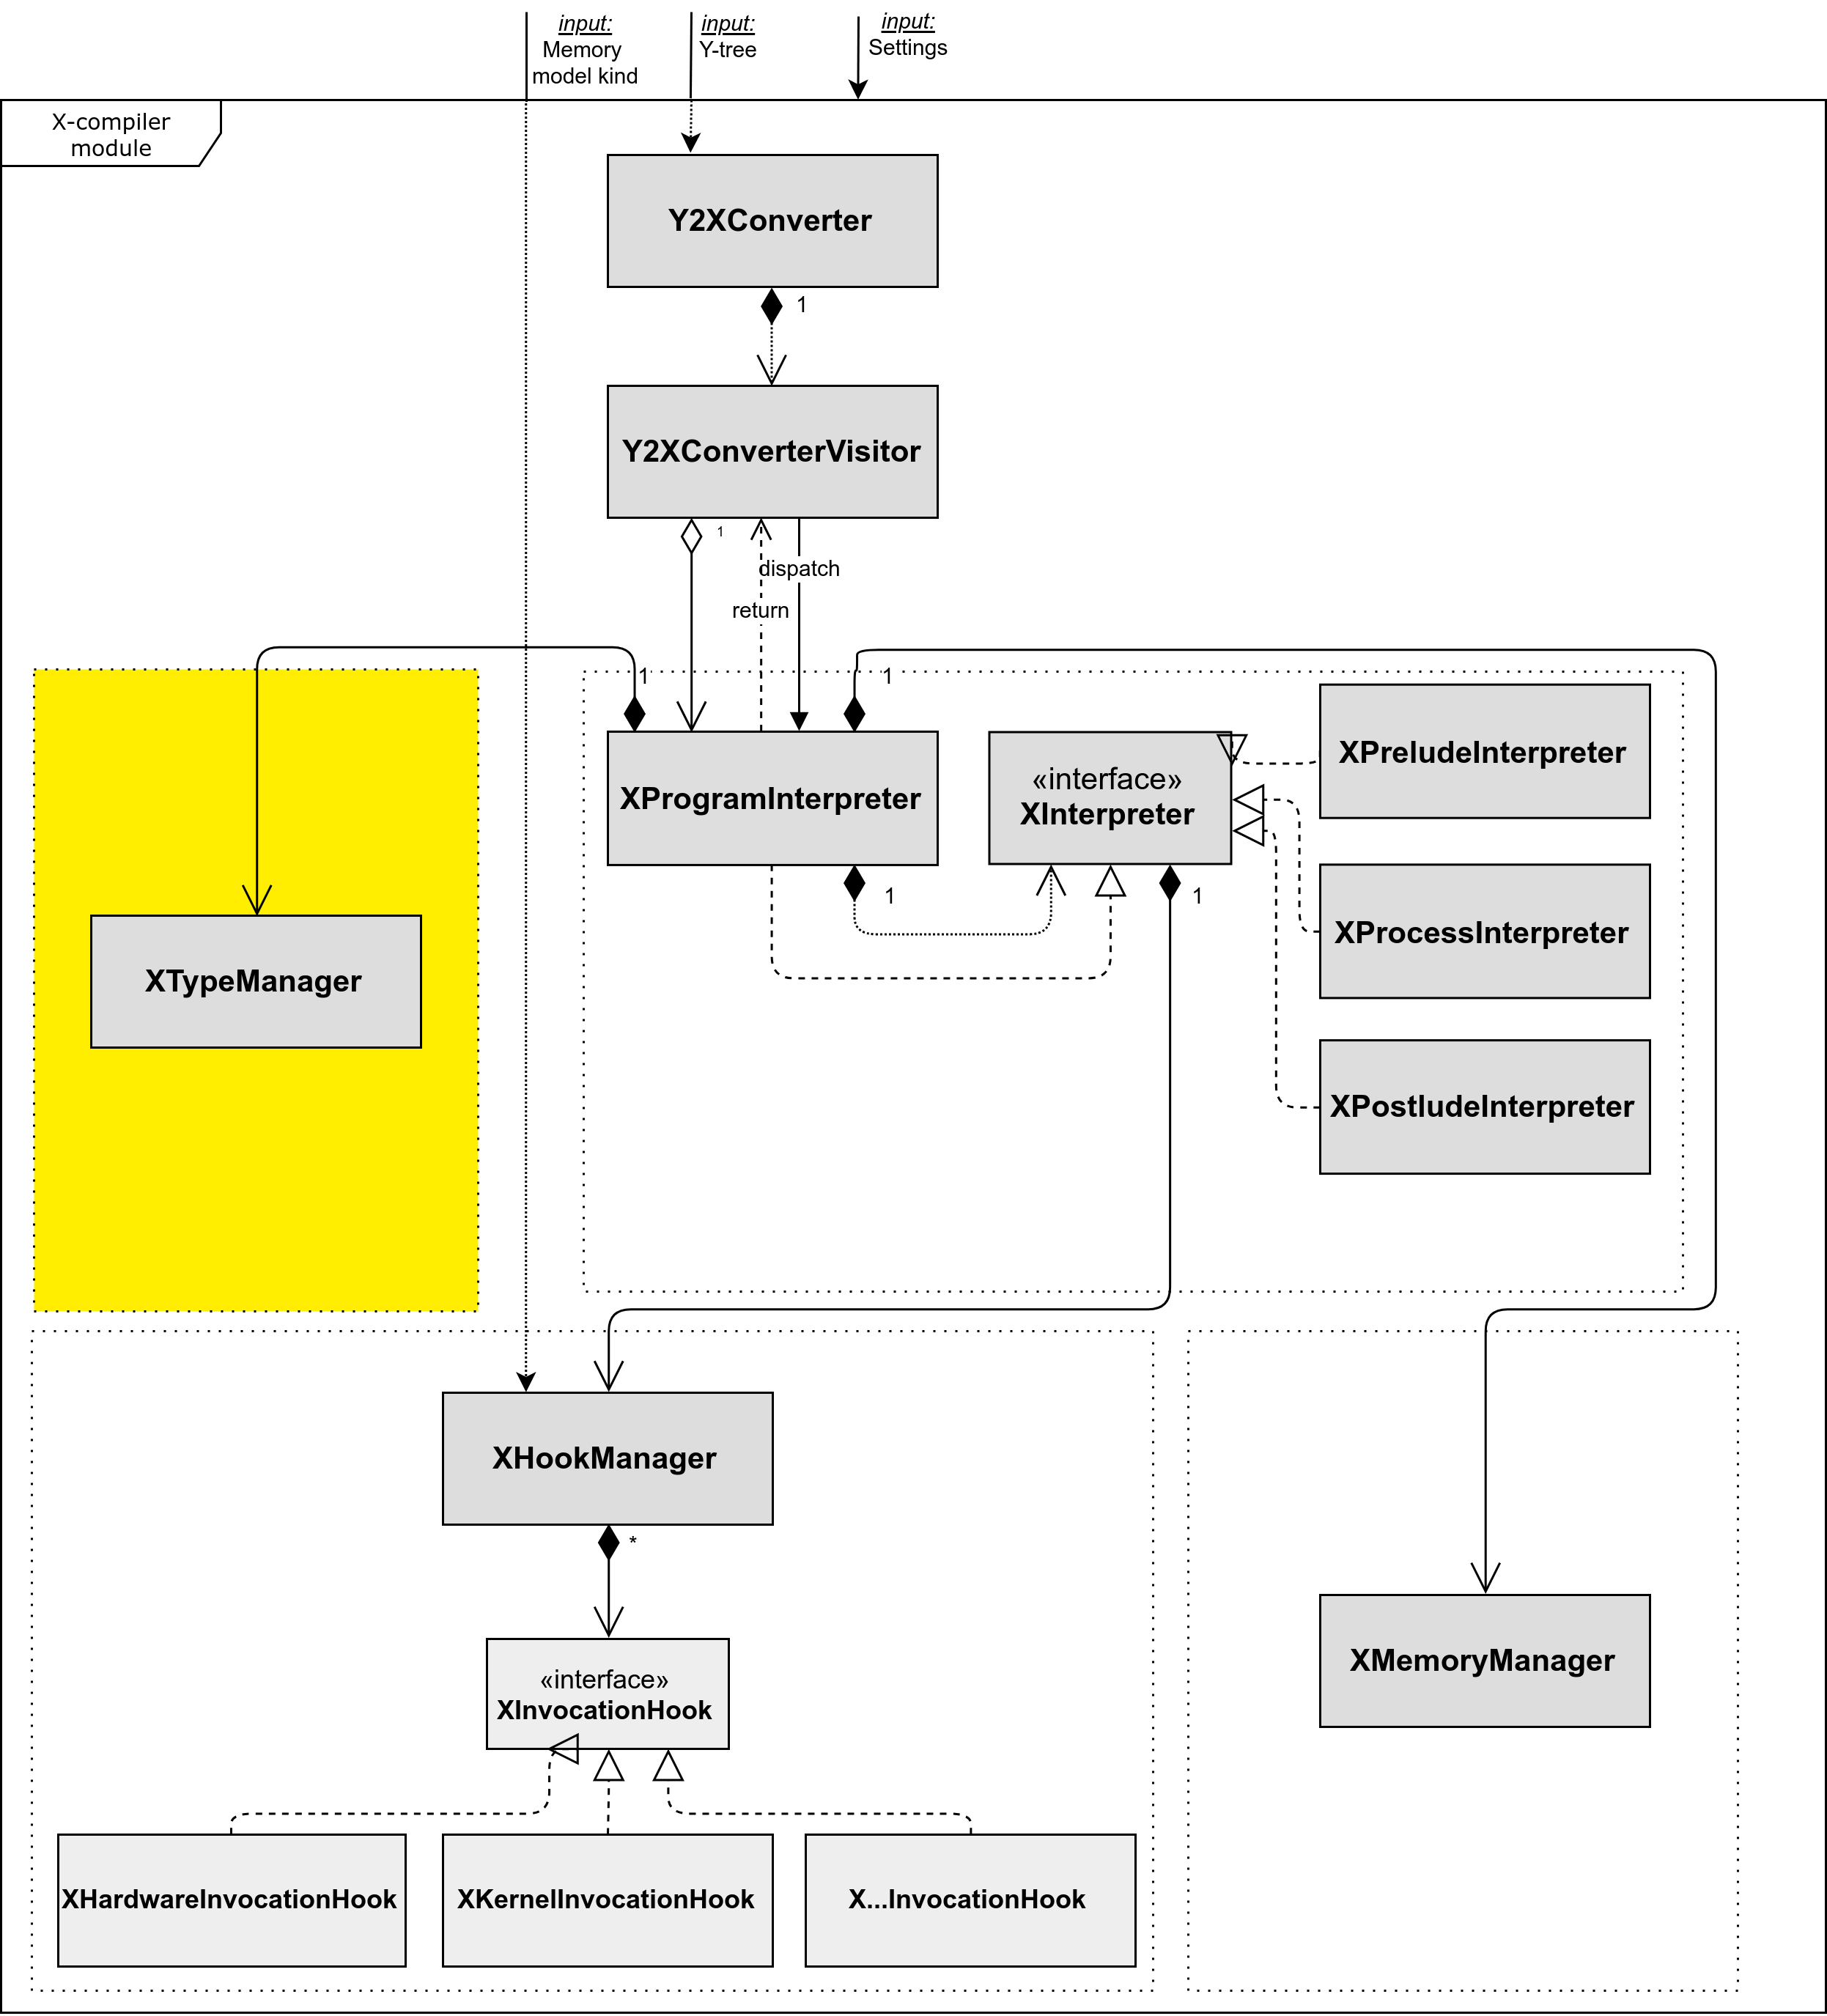
\includegraphics[height=.99\paperheight]{img/compiler/X-compiler-3.png}}
\end{figure}}
\only<5>{\begin{figure}
  \scalebox{0.9}{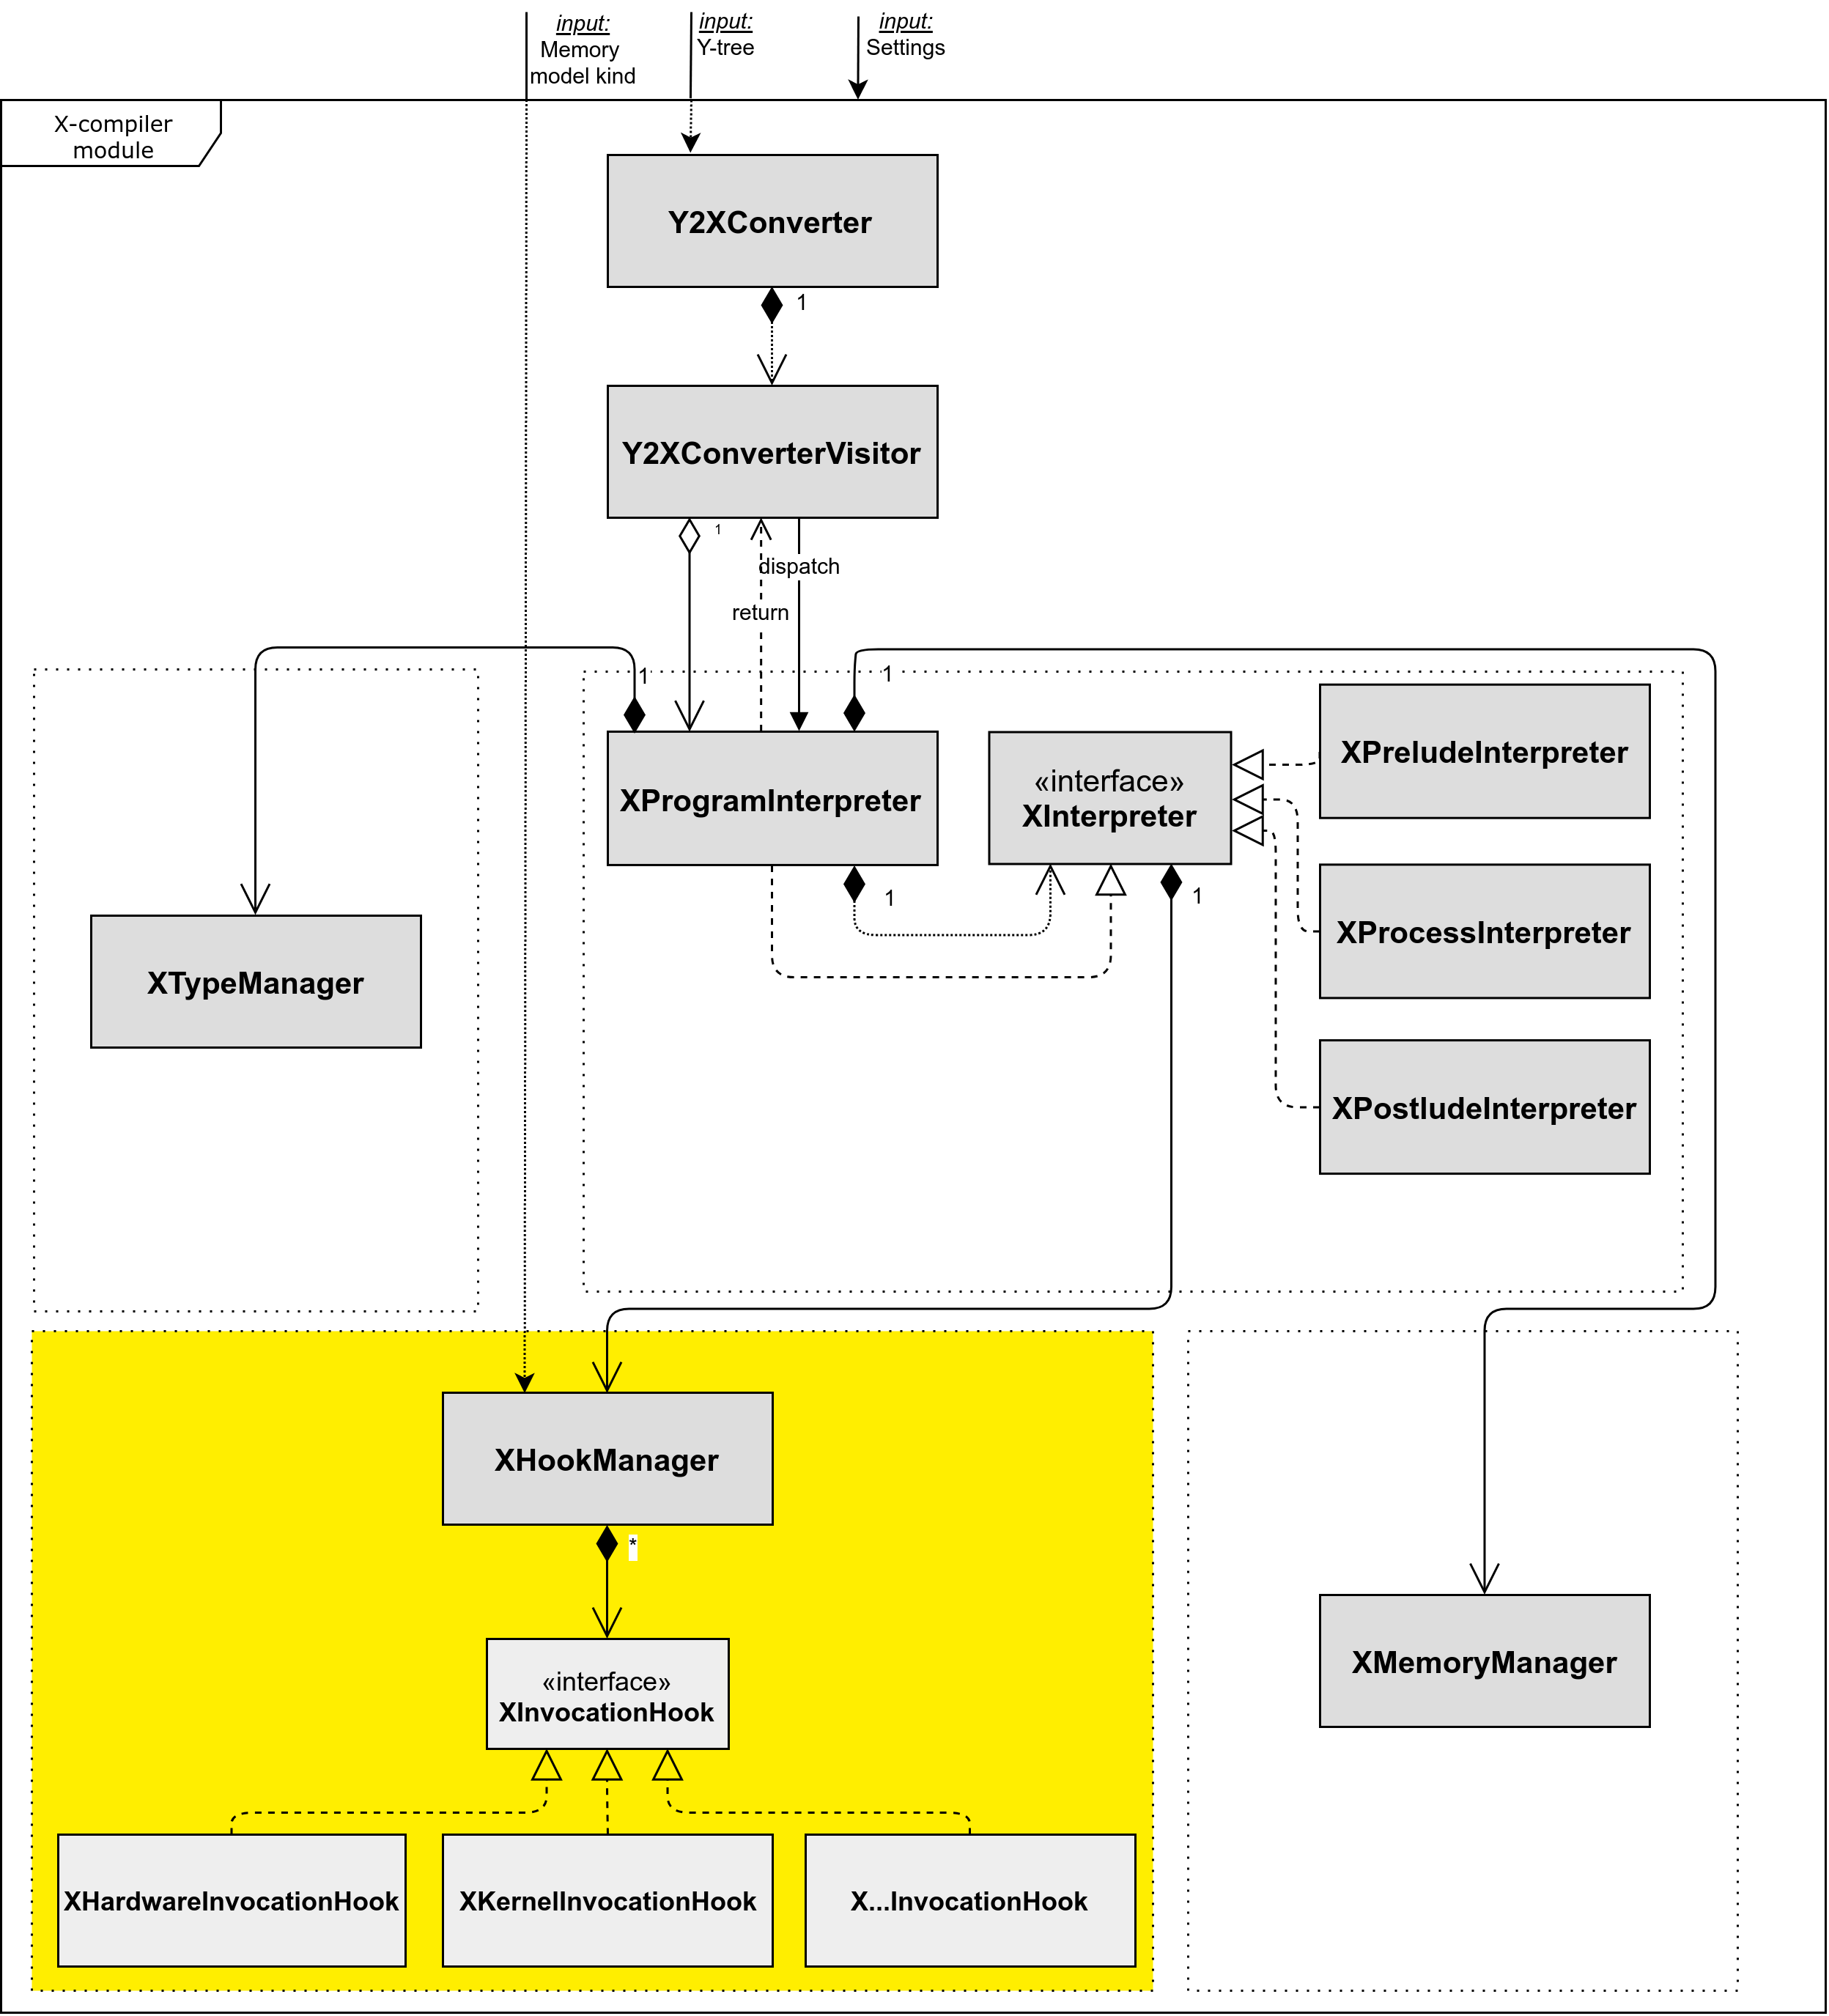
\includegraphics[height=.99\paperheight]{img/compiler/X-compiler-4.png}}
\end{figure}}
\end{minipage}
\end{frame}



\begin{frame}{\tool{Porthos\,v1}: The input language}
{
\only<1-2>{ }
\only<3>{Static syntactic determination of the variables kind}
\only<4>{Lack of support for functions invocations}
\only<5>{Lack of support for unconditional jumps}
}
{\noindent\centering
\begin{minipage}{.45\textwidth}
  \begin{figure}
  \only<1-2>{\lstinputlisting[language=Java,basicstyle=\ttfamily\tiny,columns=fullflexible]{img/lst/input-old/example-old.c}}
    \only<3>{\lstinputlisting[language=Java,basicstyle=\ttfamily\tiny,columns=fullflexible]{img/lst/input-old/example-old-2.c}}
    \only<4>{\lstinputlisting[language=Java,basicstyle=\ttfamily\tiny,columns=fullflexible]{img/lst/input-old/example-old-3.c}}
    \only<5>{\lstinputlisting[language=Java,basicstyle=\ttfamily\tiny,columns=fullflexible]{img/lst/input-old/example-old.c}}
  \caption{A program example in the \tool{Porthos\,v1} input language}
  \end{figure}
\end{minipage}
%
\begin{minipage}{.45\textwidth}
  \begin{figure}
  \only<2,5>{\lstinputlisting[basicstyle=\ttfamily\Tiny,columns=fullflexible,literate={<}{{$\langle$}}1{>}{{$\rangle$}}1,escapeinside={[*}{*]}]{img/lst/input-grammar/grammar.txt}}
  \only<3>{\lstinputlisting[basicstyle=\ttfamily\Tiny,columns=fullflexible,literate={<}{{$\langle$}}1{>}{{$\rangle$}}1,escapeinside={[*}{*]}]{img/lst/input-grammar/grammar-2.txt}}
  \only<4>{\lstinputlisting[basicstyle=\ttfamily\Tiny,columns=fullflexible,literate={<}{{$\langle$}}1{>}{{$\rangle$}}1,escapeinside={[*}{*]}]{img/lst/input-grammar/grammar-3.txt}}
  \vfill
  \only<2->{\caption{A sketch of the \tool{Porthos\,v1} input language grammar}}
  \end{figure}
\end{minipage}
}
\end{frame}


\begin{frame}[label={example-new}]{\tool{PorthosC}: The input language}
{
\only<1-2>{ }
\only<3>{Pre-compilation phase for the syntactic determination of the variables kind}
\only<4>{Support for functions invocations: The invocation hooking mechanism}
\only<5>{Support for arbitrary control-flow jumps}
}
{\noindent\centering
\begin{minipage}{.43\textwidth}
  \begin{figure}
  \only<1-2>{\lstinputlisting[language=Java,basicstyle=\ttfamily\tiny,columns=fullflexible]{img/lst/input-new/example-new.c}}
    \only<3>{\lstinputlisting[language=Java,basicstyle=\ttfamily\tiny,columns=fullflexible]{img/lst/input-new/example-new-2.c}}
    \only<4>{\lstinputlisting[language=Java,basicstyle=\ttfamily\tiny,columns=fullflexible]{img/lst/input-new/example-new-3.c}}
    \only<5>{\lstinputlisting[language=Java,basicstyle=\ttfamily\tiny,columns=fullflexible]{img/lst/input-new/example-new-4.c}}
  \caption{A program example in the \tool{Porthos\,v1} input language}
  \end{figure}
\end{minipage}
%
\begin{minipage}{.55\textwidth}
%  \only<1>{\begin{itemize}
%  \item The grammar used by \texttt{PorthosC} was taken from the C11 standard~\cite{c11}.
%  \end{itemize}}
%  %
%  \only<2>{\begin{itemize}
%    \item A variable is shared if:
%      \begin{itemize}
%      \item it was declared as a \textit{pointer}, or
%      \item its \textit{address} is accessed at least once by the code of any process, or 
%      \item it was declared as a \textit{parameter} of the function that defines a process, or 
%      \item it was exported by the \textit{extern} keyword or an exporting function.
%      \end{itemize}
%    \end{itemize}
%  }
%  \only<3>{\begin{itemize}
%    \item The invocation hooking mechanism serves as an extensible knowledge base for storing the semantics of functions.
%    \end{itemize}
%  }
%  \only<4>{\begin{itemize}
%    \item The labels are being collected during the pre-compilation stage,
%    \item the jumps are being resolved during the compilation.
%    \end{itemize}
%  }  \scalebox{0.75}{\includegraphics[height=\textheight,keepaspectratio]{img/lst/input-new/t0-3.png}}
%  }
%  \only<5>{
%    \scalebox{0.75}{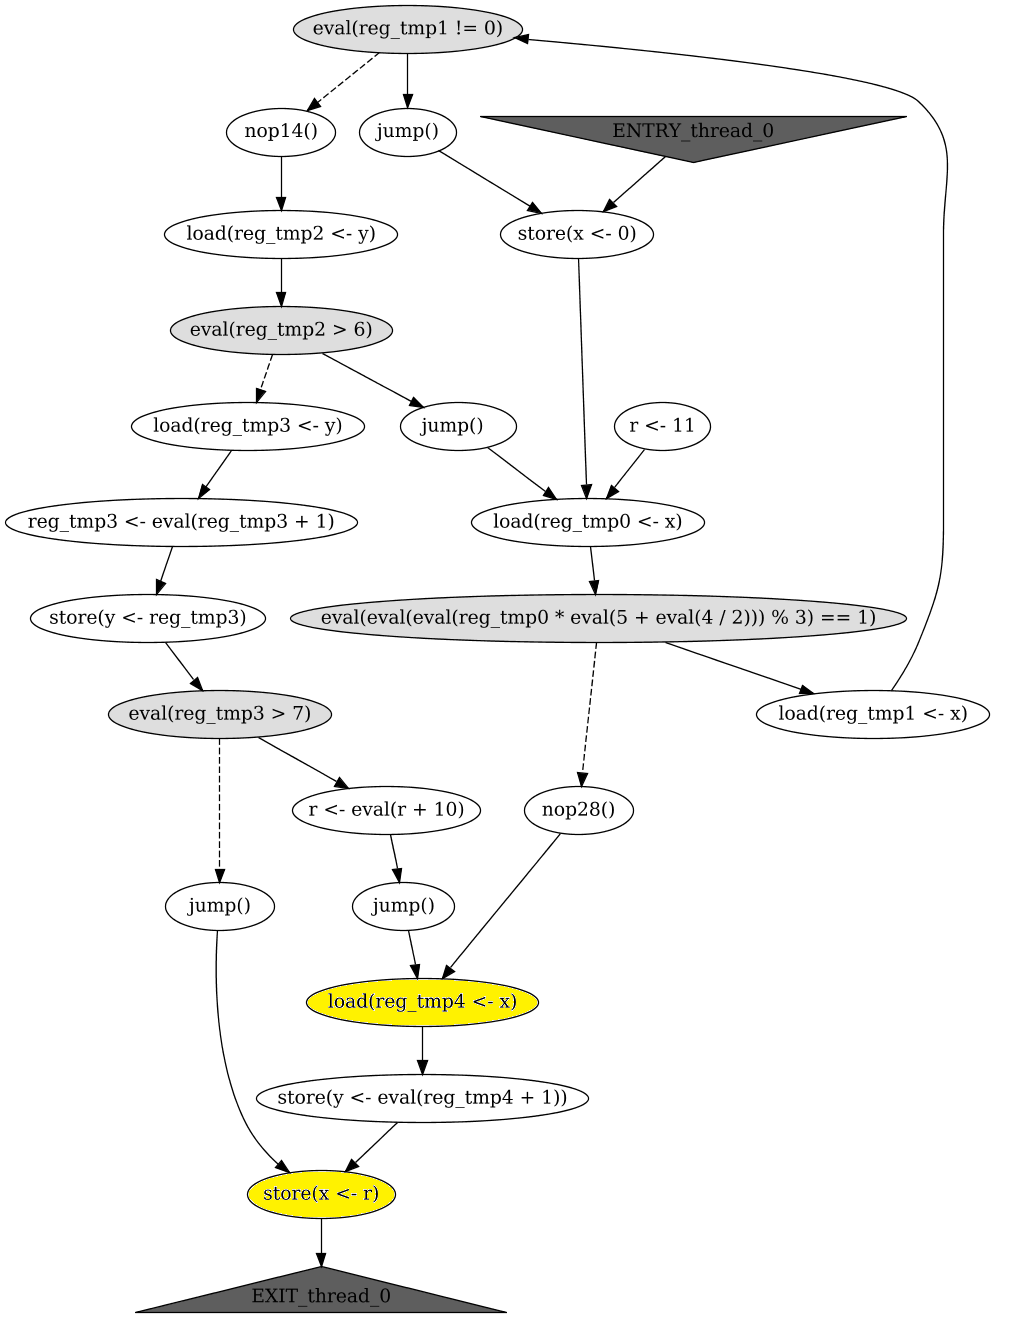
\includegraphics[height=\textheight,keepaspectratio]{img/lst/input-new/t0-4.png}}
%  }
  \begin{figure}
  \only<2-3>{
    \scalebox{0.75}{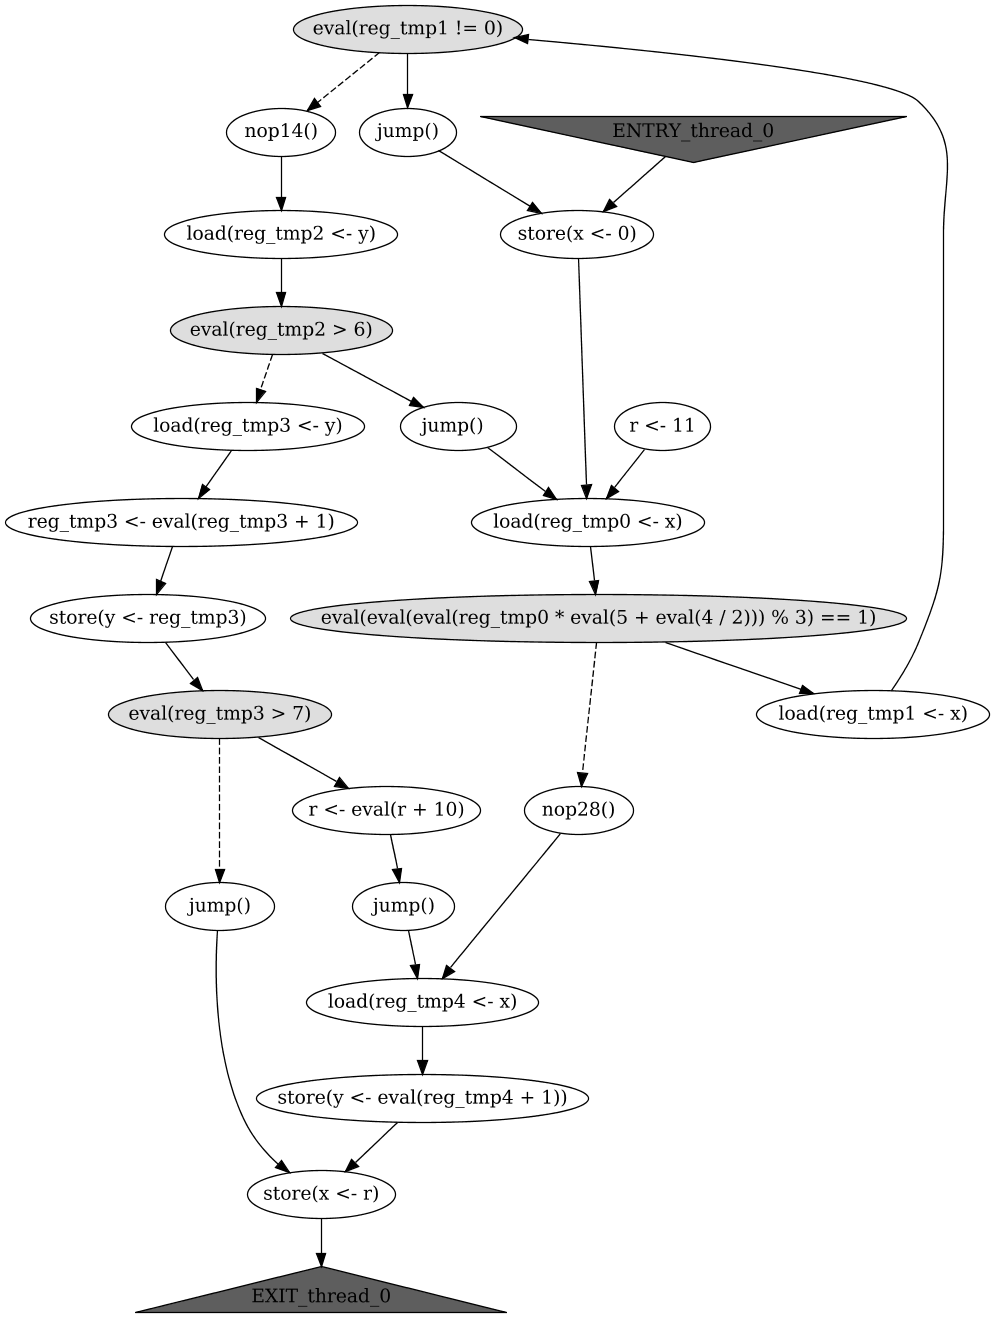
\includegraphics[height=\textheight,keepaspectratio]{img/lst/input-new/t0.png}}
  }
  \only<4>{
    \scalebox{0.75}{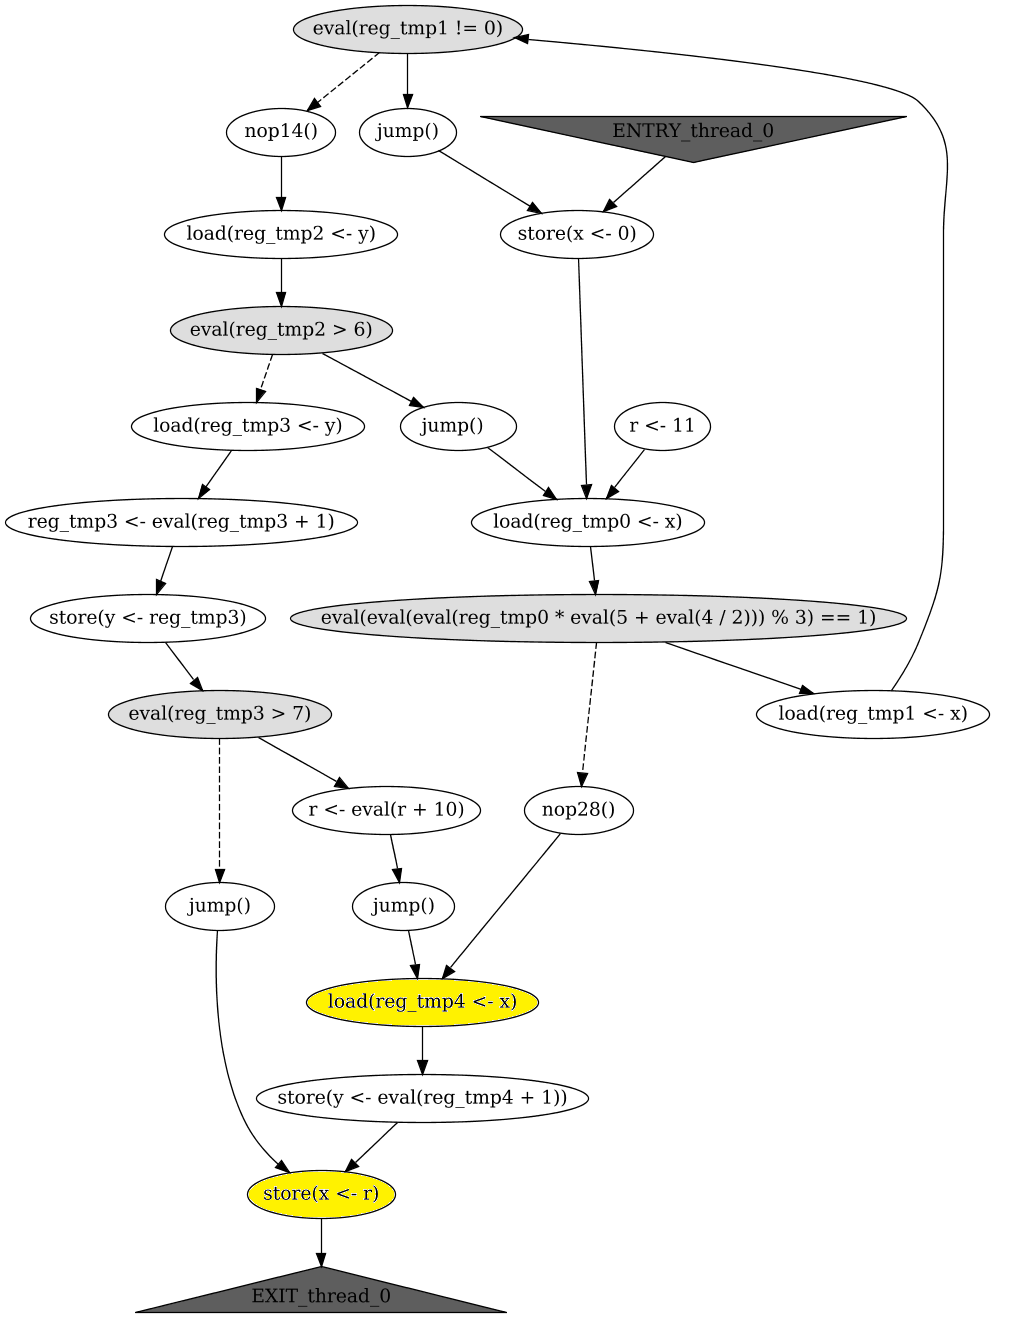
\includegraphics[height=\textheight,keepaspectratio]{img/lst/input-new/t0-4.png}}
  }
  \only<5>{
    \scalebox{0.75}{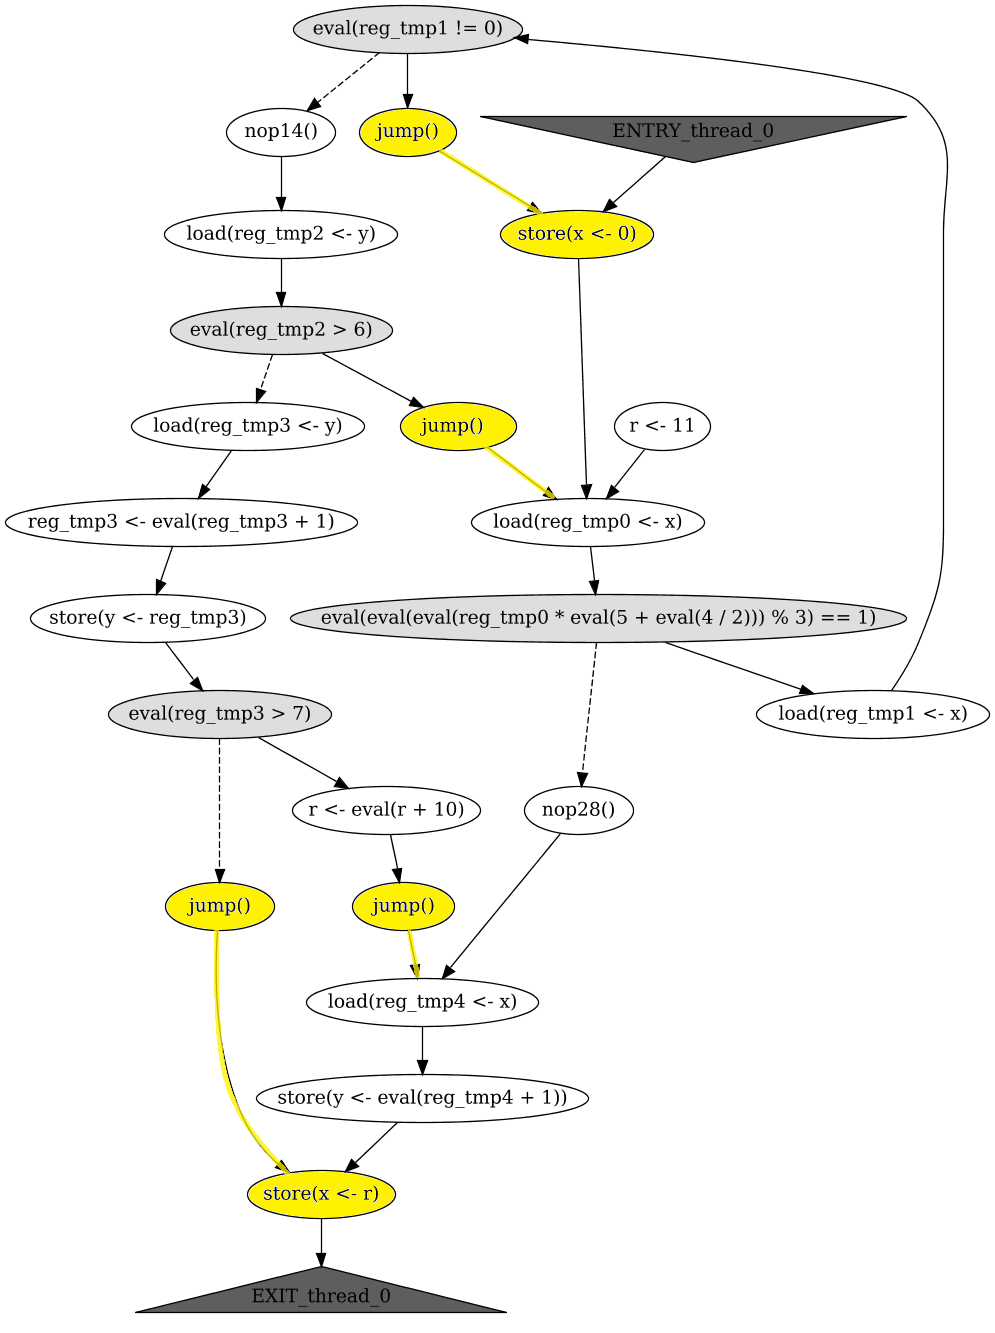
\includegraphics[height=\textheight,keepaspectratio]{img/lst/input-new/t0-5.png}}
  }
  \only<2->{\caption{The compiled event-flow graph}}
  \end{figure}
\end{minipage}
}
\end{frame}


\begin{frame}{\texttt{PorthosC}: The new control-flow encoding scheme}
\begin{figure}
\begin{minipage}{.2\textwidth}
\centering
\begin{tikzpicture}[->,>=stealth',shorten >=1pt,auto,node distance=1.5cm,semithick]
    \node[c] (i)   [] {$e_1$};
    \node[c] (ii)  [below of=i] {$e_2$};
    \node[c,fill=black!15] (lnop) [below left = 0.25cm and 0.7cm of ii] {$e_{nop_{1}}$};
    \node[c] (iii) [below of=ii] {$e_3$};
    \node[c,fill=black!15] (rnop) [right = 0.4cm of iii] {$e_{nop_{2}}$};
    \node[c] (iv)  [below of=iii] {$e_4$};
    \path[->]
    (i) edge [right] node {$\epsilon$} (ii)
    (i) edge [right,bend right=25] node {$g_{1,4}$} (lnop)
    (lnop) edge [right,bend right=25] node {$\epsilon$} (iv)
    (ii) edge [right] node {$g_{2,3}$} (iii)
    (iii) edge [right] node {$\epsilon$} (iv)
    (ii) edge [right,bend left=25] node {$g_{2,4}$} (rnop)
    (rnop) edge [right,bend left=25] node {$\epsilon$} (iv)
    ;
\end{tikzpicture}
\end{minipage}
%
\hspace{15pt}
\begin{minipage}{.4\textwidth}
\centering
\begin{align*}
\phi_{CF} \defeq \ & [\fx(e_2) \Rightarrow \fx(e_1)] \\
                 \ & \land [\fx(e_3) \Rightarrow \fx(e_2)] \\
                 \ & \land [\fx(e_{nop_{1}}) \Rightarrow \fx(e_1)] \\
                 \ & \land [\fx(e_{nop_{2}}) \Rightarrow \fx(e_2)] \\
                 \ & \land [\fx(e_4) \Rightarrow (\fx(e_{nop_{1}}) \lor \fx(e_3) \lor \fx(e_{nop_{2}}))] \\
                 \ & \land [\fx(e_{nop_{1}}) \land \fx(e_1) \Rightarrow g_{1,4}] \\
                 \ & \land [(\fx(e_3) \land \fx(e_2)) \Rightarrow g_{2,3}] \\
                 \ & \land [(\fx(e_{nop_{2}}) \land \fx(e_2)) \Rightarrow g_{2,4}] \\
                 \ & \land \lnot [\fx(e_2) \land \fx(e_{nop_{1}})] \\
                 \ & \land \lnot [\fx(e_3) \land \fx(e_{nop_{2}})]
\end{align*}
\end{minipage}
\caption{Example of encoding for the control-flow of the event-flow graph}
\end{figure}
\end{frame}



\begin{frame}<presentation:0>{Encoding for the data-flow}
\begin{itemize}
\item SSA-indices are computed as following:
\begin{itemize}
  \item any access to a shared variable (both read and write) increments its SSA-index;
  \item only writes to a local variable increment its SSA-index (reads preserve indices);
  \item no access to a constant variable or computed (evaluated) expression changes their SSA-index.
\end{itemize}
\end{itemize}
The data-flow of an event is encoded as following:
\begin{align}
    \phi_{DF_{e = \texttt{load}(r \leftarrow l)}}  \defeq \ & [\fx(e) \Rightarrow (r_{i+1} = l_{i+1})] \nonumber \\
    \phi_{DF_{e = \texttt{store}(l \leftarrow r)}} \defeq \ & [\fx(e) \Rightarrow (l_{i+1} = r_i)] \nonumber\\
    \phi_{DF_{e = \texttt{eval}(\cdot)}}           \defeq \ & [\fx(e) \Rightarrow \fv(e)] \nonumber \\
\end{align}
%    \phi_{DF_{mem}}(e_1, e_2) \defeq \ & [\texttt{rf}(e_1, e_2) \Rightarrow (l_i = l_j)] \nonumber
\end{frame}



\begin{frame}{\texttt{PorthosC}: The new DFS-based \texttt{X-graph} unrolling scheme}
\only<1>{
\begin{figure}[t]
\centering
\resizebox{.8\linewidth}{!}{
\begin{tikzpicture}[->,>=stealth',shorten >=1pt,auto,node distance=1.5cm,semithick]
\node[c] (1) [] {$1$};
\node[c] (2) [below left of=1] {$2$};
\node[c] (3) [below right of=1] {$3$};
\node[c] (4) [below of=3] {$4$};
\path[->]
(1) edge [] node {} (2)
(2) edge [bend left=50,dotted] node {} (1)
(1) edge [] node {} (3)
(3) edge [] node {} (4)
(4) edge [bend right=80,dotted] node {} (1)
;
\node[draw=none] (impl) [right=3cm of 3] {$\overset{k = 6}{\longmapsto}$};
;
\node[c] (22) [right=3cm of impl] {$2_2$};
\node[c] (11) [above right=1cm and 1cm of 22]{$1_1$};
\node[c] (32) [below right=1cm and 1cm of 11] {$3_2$};
\node[c] (43) [below of=32] {$4_3$};
\node[c] (13) [below of=22] {$1_3$};
\node[c] (24) [below left=1cm and 1cm of 13] {$2_4$};
\node[c] (34) [below right=1cm and 1cm of 13] {$3_4$};
\node[c] (14) [below of=43] {$1_4$};
\node[c] (15) [below of=24] {$1_5$};
\node[c] (45) [below of=34] {$4_5$};
\node[c] (25) [below of=14] {$2_5$};
\node[c] (35) [below of=14] {$3_5$};
\node[c] (26) [below left=1cm and 1cm of 15] {$2_6$};
\node[c] (36) [below right=1cm and 1cm of 15] {$3_6$};
\node[c] (16) [below right=1cm and 0.2cm of 45] {$1_6$};
\node[c] (46) [below right=1cm and 0.3cm of 35] {$4_6$};
\node[rectangle,draw] (6) [below left=1cm and 1cm of 16] {$S$};
\node[] (k1) [right=3.2cm of 11] {$(k = 1)$};
\node[] (k2) [right=1.7cm of 32] {$(k = 2)$};
\node[] (k3) [right=1.7cm of 43] {$(k = 3)$};
\node[] (k4) [right=1.7cm of 14] {$(k = 4)$};
\node[] (k5) [right=1.7cm of 35] {$(k = 5)$};
\node[] (k6) [right=1cm of 46] {$(k = 6)$};
\path[->]
(11) edge [] node {} (22)
(11) edge [] node {} (32)
(32) edge [] node {} (43)
(22) edge [] node {} (13)
(13) edge [bend right=10] node {} (24)
(13) edge [bend left=10] node {} (34)
(43) edge [] node {} (14)
(24) edge [] node {} (15)
(34) edge [] node {} (45)
(14) edge [] node {} (25)
(14) edge [] node {} (35)
(15) edge [bend right=10] node {} (26)
(15) edge [bend left=10] node {} (36)
(45) edge [] node {} (16)
(35) edge [bend right=10] node {} (16)
(35) edge [bend left=10] node {} (46)
(26) edge [bend right=10] node {} (6)
(36) edge [bend right=5] node {} (6)
(16) edge [bend left=20] node {} (6)
(46) edge [bend left=20] node {} (6)
;
\end{tikzpicture}
}
\caption{Example of the flow graph unrolling up to bound $k = 6$}
\end{figure}
}
%
%\only<2>{
%\begin{figure}
%  \scalebox{0.8}{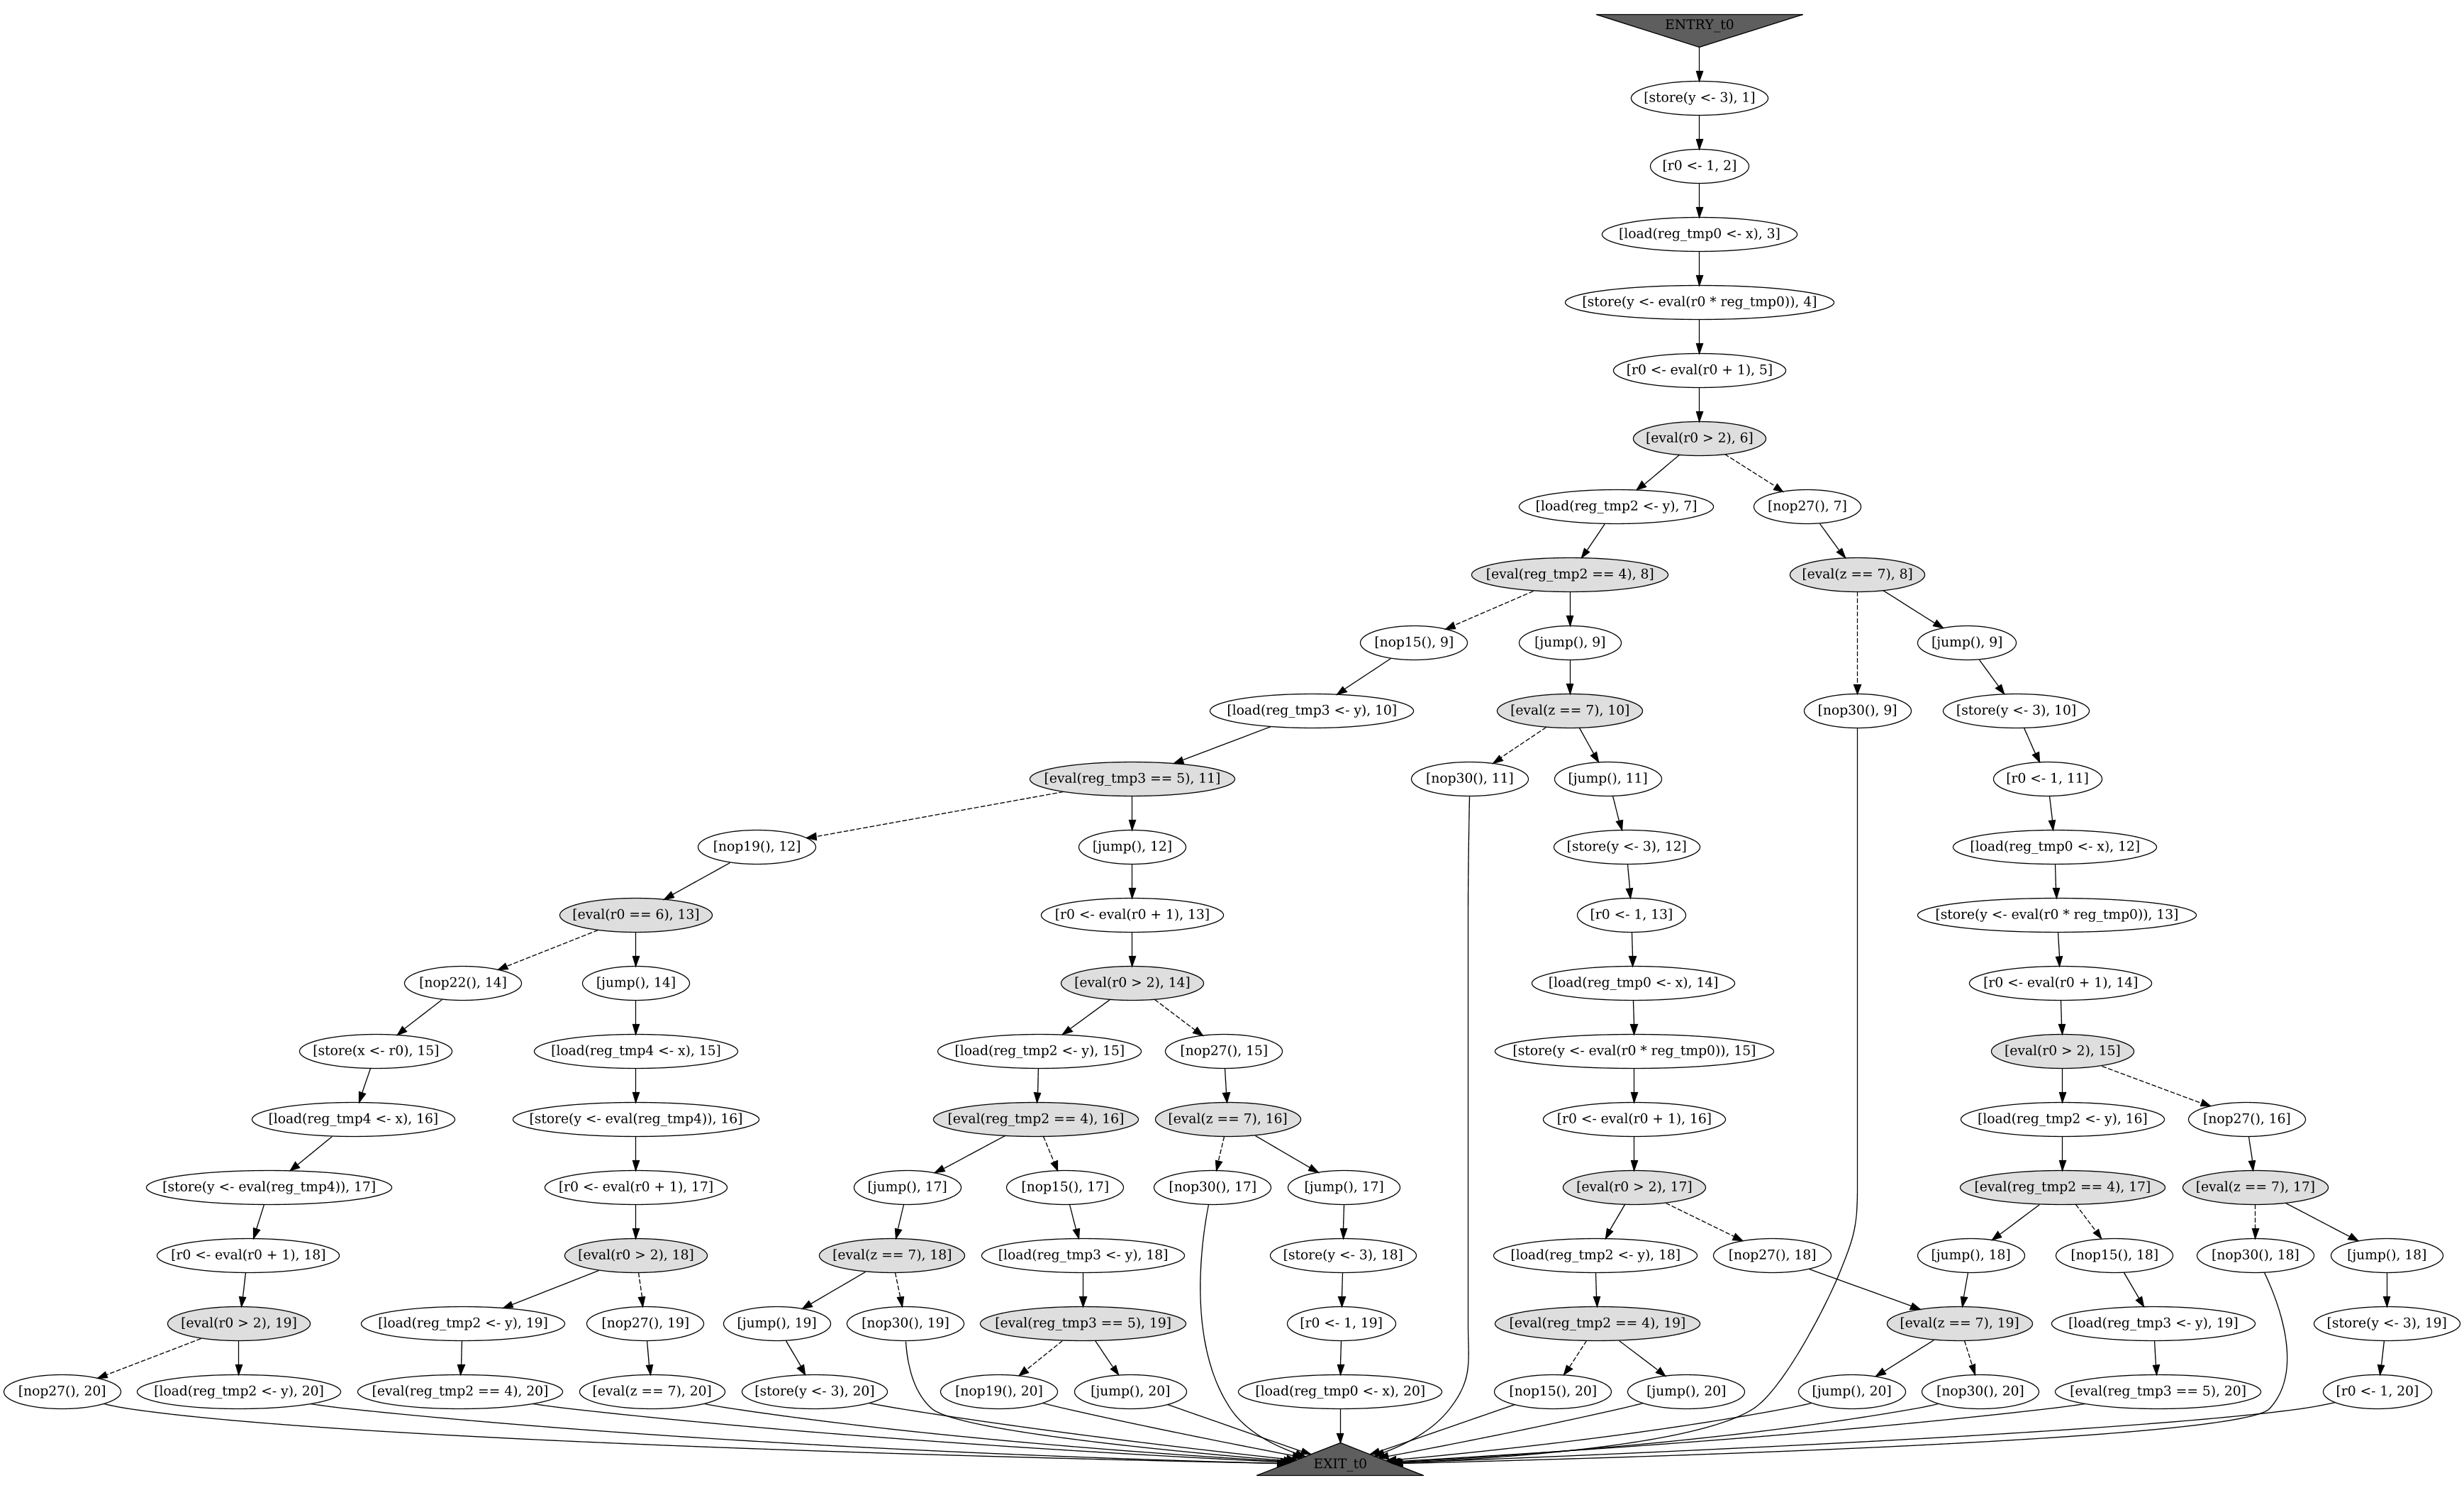
\includegraphics[height=\textheight,keepaspectratio]{img/lst/input-new/t0_unrolled.png}}
%  \caption{The unrolled \texttt{X-graph} of the code used on slide~\ref{example-new}}
%\end{figure}
%}
\end{frame}



\begin{frame}{Evaluation}{The new unrolling scheme}
\begin{minipage}{.23\linewidth}
\hfill
\end{minipage}
%
\noindent\begin{minipage}{.75\linewidth}
\begin{figure}
  \vspace{-20pt}
  \centering
  \scalebox{.8}{
    \colorbox{white}{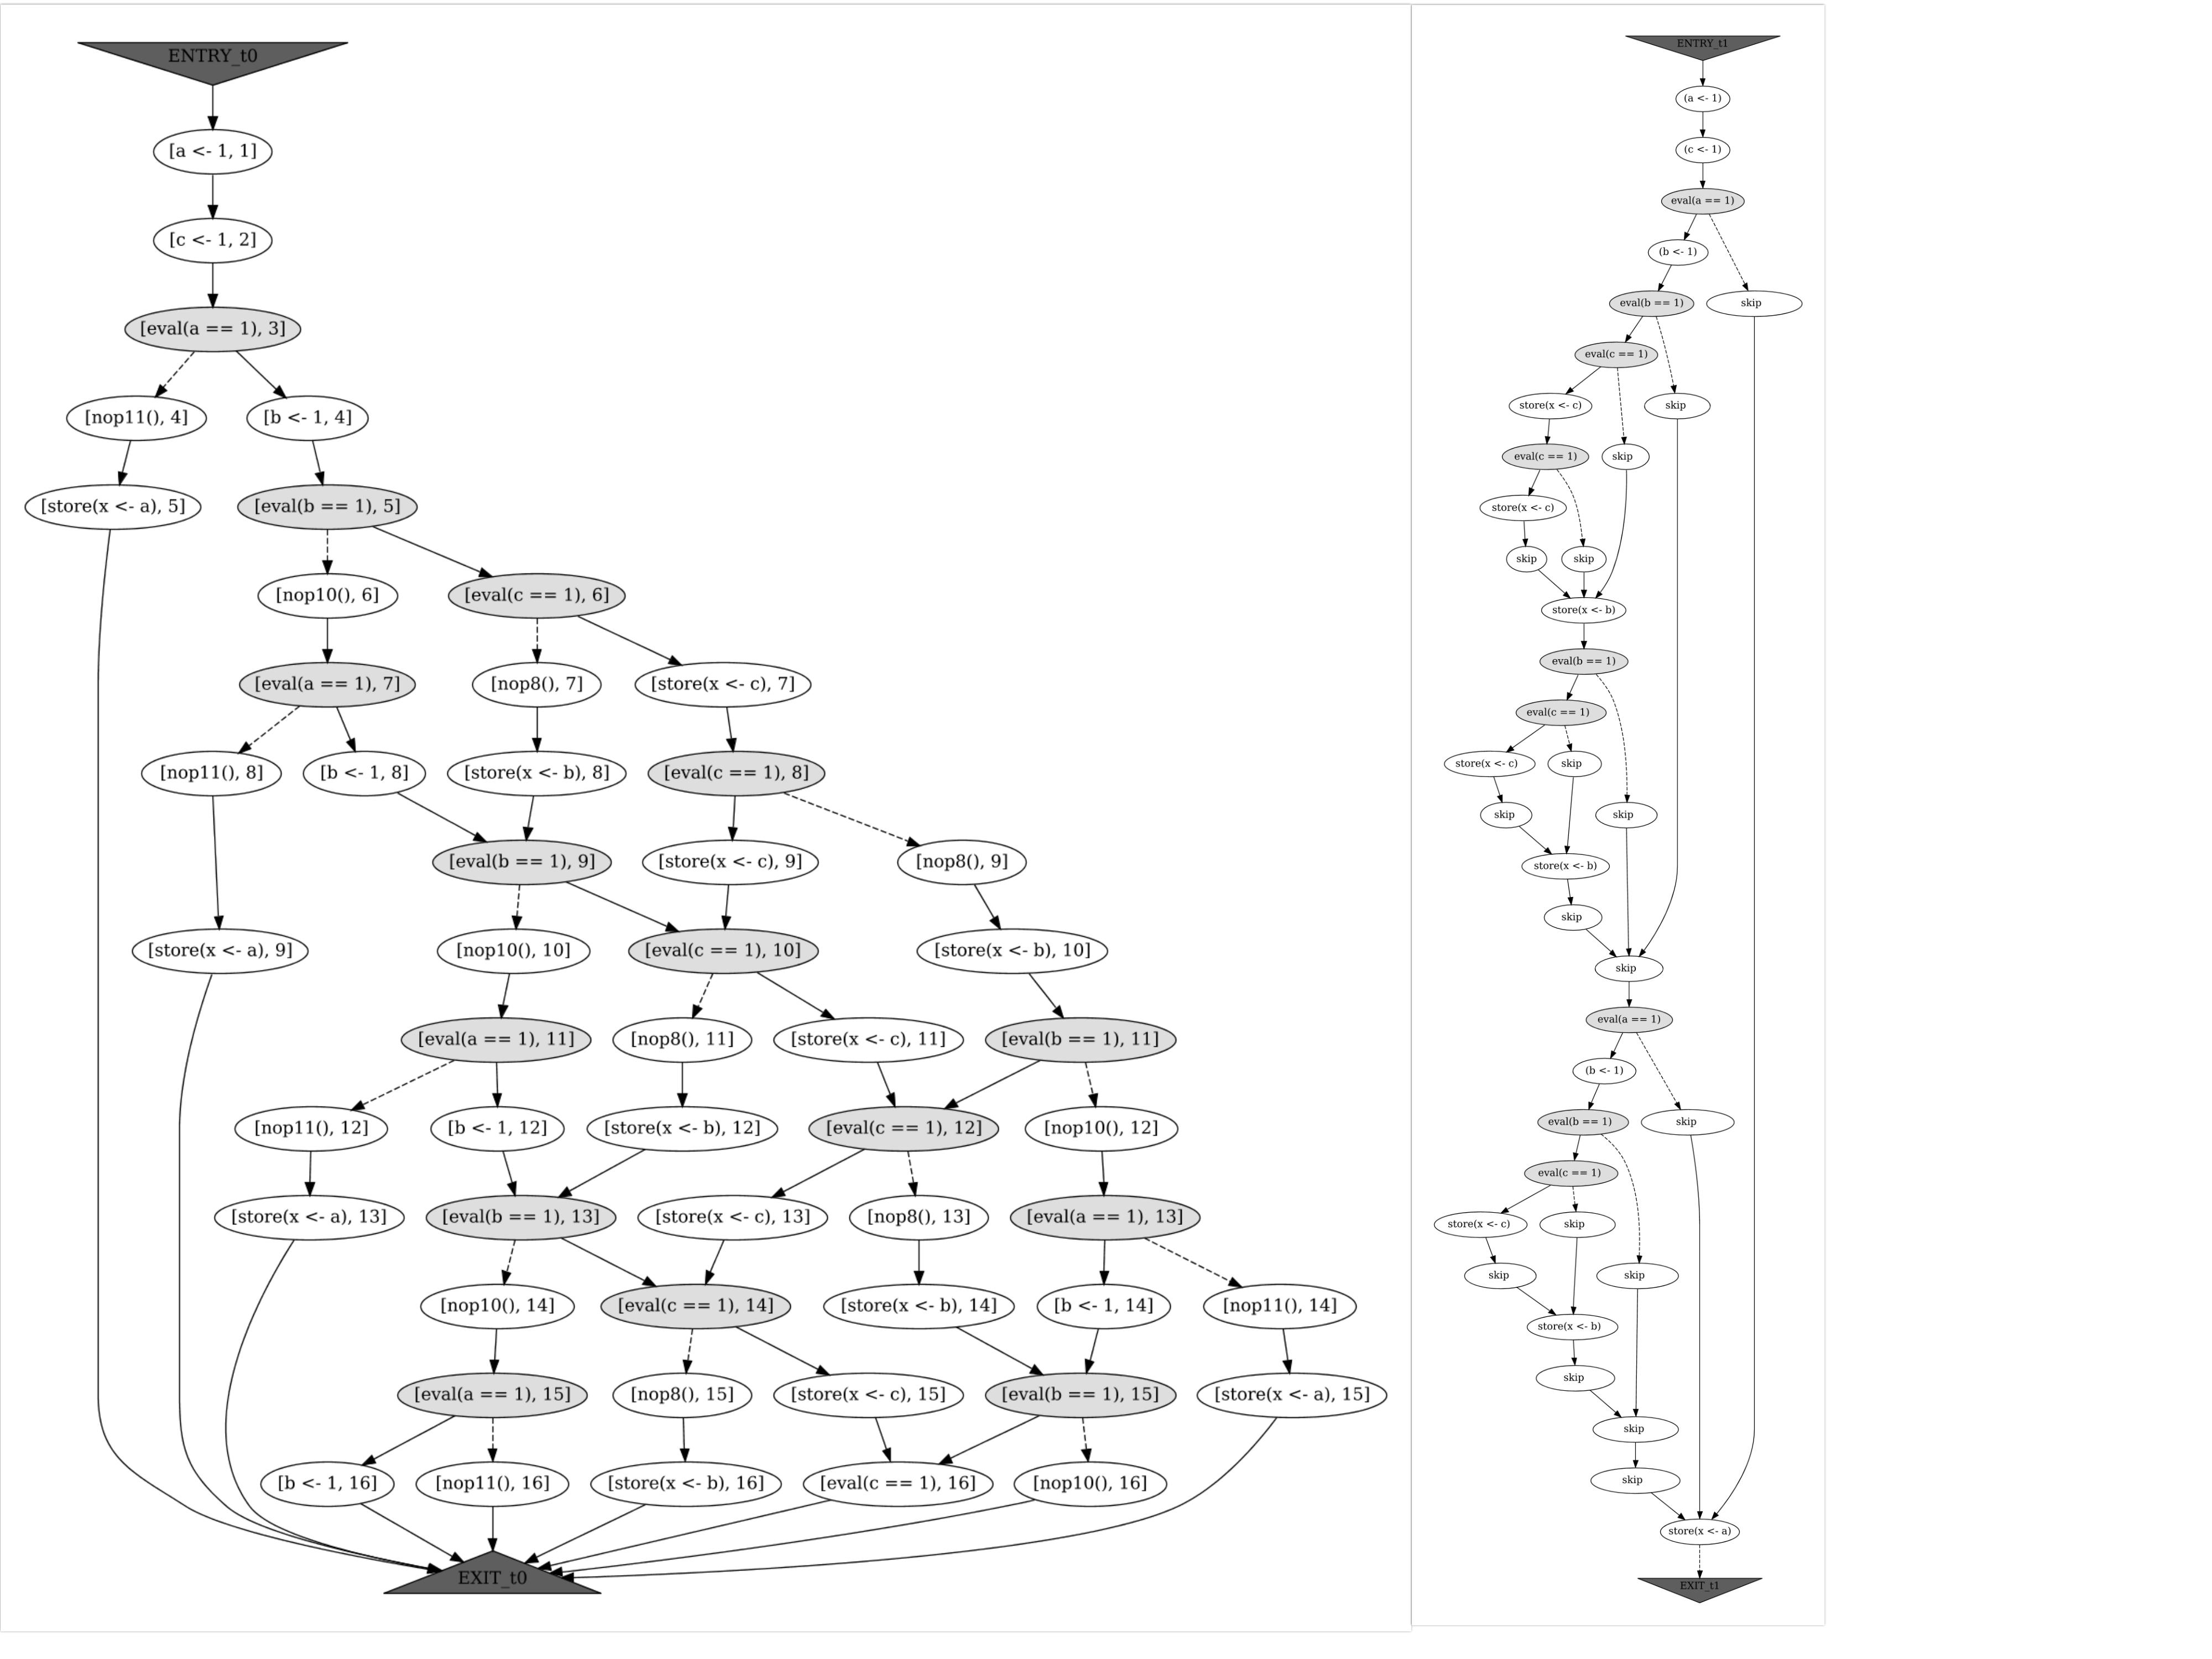
\includegraphics[height=\textheight,keepaspectratio]{img/lst/unrolled/collage.jpg}}
  }
\caption{Illustration of differences in unrolling schemes of \tool{PorthosC}~(left) and \tool{Porthos\,v1}~(right)}
\end{figure}
\end{minipage}
\end{frame}


\begin{frame}{Evaluation}{Overhead of the new unrolling scheme: Number of events}
\begin{figure}[t]
\begin{subfigure}{.47\textwidth}
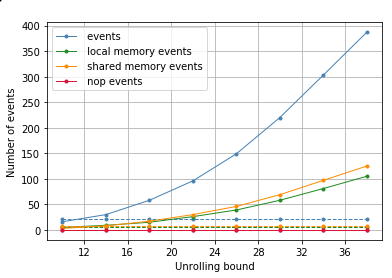
\includegraphics[width=\textwidth,keepaspectratio]{../img/my/performance/new/new-e.png}
\caption{The graph unrolled by \tool{PorthosC}}
\label{dep:events:new}
\end{subfigure}
\hfill
%
\begin{subfigure}{.47\textwidth}
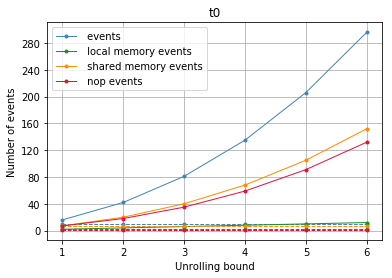
\includegraphics[width=\textwidth,keepaspectratio]{../img/my/performance/new/old-e.png}
\caption{The graph unrolled by \tool{Porthos\,v1}}
\label{dep:events:old}
\end{subfigure}
%
\caption{Dependency of unrolled events number on the unrolling bound $k$}
\label{dep:events}
\end{figure}
\end{frame}


\begin{frame}{Evaluation}{Overhead of the new unrolling scheme: Execution time}
\begin{figure}[t]
\begin{subfigure}{.45\textwidth}
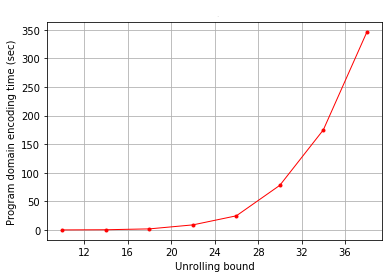
\includegraphics[width=\textwidth,keepaspectratio]{../img/my/performance/new/new-t.png}
\caption{Program domain encoding time of the graph unrolled by \tool{PorthosC}}
\label{dep:time:new}
\end{subfigure}
\hfill
%
\begin{subfigure}{.45\textwidth}
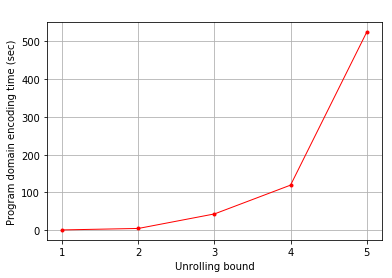
\includegraphics[width=\textwidth,keepaspectratio]{../img/my/performance/new/old-t.png}
\caption{Program domain encoding time of the graph unrolled by \tool{Porthos\,v1}}
\label{dep:time:old}
\end{subfigure}
%
\caption{Dependency of program domain encoding time (in seconds) on the unrolling bound}
\label{dep:time}
\end{figure}
\end{frame}

%\section*{Summary}

\begin{frame}{Summary}
\begin{itemize}
\item The result of the work is the generalised framework for memory model-aware analysis \textbf{\tool{PorthosC}};
  \begin{itemize}
  \item The \textit{input language} has been extended to a higher subset of C language (including unconditional control-flow jumps);
  \item The old \textit{architecture} of \texttt{Porthos} has been revised and redesigned for \texttt{PorthosC};
  \item The \textit{new unrolling scheme} produces complete state space of the analysing program within the user-defined bound $k$, though the encoding time growth rapidly (exponentially) as the unrolling bound grows.
  \item The \textit{invocation hooking mechanism} serves as a knowledge base for the program domain, it is to be filled and extended in future.
  \end{itemize}
\end{itemize}
\end{frame}


\begin{frame}{Directions for future work}
\begin{itemize}
\item Extending the \textit{knowledge base} of domain-specific functions to model synchronisation primitives;
\item Supporting \textit{new input languages} (e.g., different assembly languages);
\item Supporting \textit{complex data types} (s.a. arrays, pointers, structures, etc.);
\item Adding the \textit{inter-procedural analysis mode};
\item Handling the \textit{state explosion problem} (with standard model-checking techniques adjusted by the information about the weak memory model of the execution environment).
\end{itemize}
\end{frame}


% All of the following is optional and typically not needed. 
\appendix
\section<presentation>*{\appendixname}
\subsection<presentation>*{For Further Reading}

\begin{frame}[allowframebreaks]
  \frametitle<presentation>{Bibliography}
  \printbibliography
\end{frame}

\end{document}


